\documentclass{article}
\usepackage{geometry}
\usepackage{amsmath}
\usepackage{amsthm}
\usepackage{amssymb}
\usepackage{graphicx}
\usepackage{hyperref}
\usepackage{xcolor}
\usepackage{esvect}
\usepackage[shortlabels]{enumitem}

\usepackage[caption=false]{subfig}
\usepackage{zymacros}
\newcommand{\red}[1]{{\color{red}#1}}
\newcommand{\bl}[1]{{\color{blue}#1}}
\newcommand{\pl}[1]{{\color{purple}#1}}
%%%%%%%%%%%%%%%%%%%%%%%
% \NewDocumentCommand{\tens}{t_}
%  {%
%   \IfBooleanTF{#1}
%   {\tensop}
%   {\otimes}%
%  }
% \NewDocumentCommand{\tensop}{m}
%  {%
%   \mathbin{\mathop{\otimes}\displaylimits_{#1}}%
%  }

%%%%%%%%%%%%%%%%%%%%%%%%%

\begin{document}

\title{A unified framework classifying two-layer neural networks into distinct parameter regimes}
\author{}

\maketitle
%\date{\today}
\begin{abstract}
    Theoretical and empirical studies establish various understanding on deep neural networks (DNNs), in which different studies consider different pre-factor on network formulations and different parameter initialization. In this study, we propose a unified framework---that transforms different settings into a standard form---to study gradient descent (GD) behavior of two-layer neural networks (NN) as the neuron number goes to infinity. Empirically, We found a quantity consistently classify two-layer NNs into two distinct parameter regime, a linear regime and a sparsity regime. In the linear regime, with both empirical and theoretical study, we show that  parameters of two-layer NNs after training are close to their initial values, thus, the NN during training can be well approximated by the first order expansion at the initial values, i.e., a linear evolution characterized by a neural tangent kernel. We further prove that in this linear regime, two-layer NNs find the global optima exponentially fast.  In the sparsity regime, after training, a part of neurons have large weights while others keep their weights close to initial amplitudes. Our empirical studies also suggest that the sparsity amplifies and the regime boundary asymptotically goes sharp as the neuron number goes infinity. Although the current works are based on shallow networks and synthetic data, the unified framework and the two distinct regimes pave a research framework for future study on general networks and real dataset and understanding their characteristics in both regimes.
\end{abstract}

\section{Introduction}
Deep learning, an important method of modern machine learning, is often realized by a deep neural neural network (DNN), which has universal approximation ability for any continuous function as the width is sufficiently wide \cite{cybenko1989approximation}. To understand the success \cite{lecun_deep_2015} or failure \cite{nye2018efficient} of deep learning, it calls for understanding DNNs with gradient-based training. Recent years, among many, we list two approaches that have gained much understanding to this aspect.

One approach is from the perspective of the gradient flow of parameters. With different pre-factors or different initialization, many studies probe various behavior of DNNs. Consider a two-layer neural network (NN) with $m$ hidden neurons and input $\vx$
\begin{equation}
    f_{\vtheta}(\vx) = \alpha\sum_{j=1}^{m}a_j\sigma(\vw_j^\T\vx+b_j),     \label{eq: 2LNN}
\end{equation}
where $\alpha$ is the pre-factor, $\vtheta=\{(a_j,\vw_j,b_j)\}_{j=1}^{m}$ is the set of parameters. In practical training, good generalization results can often be achieved by taking the pre-factor as $1$ and initializing parameters by some common methods, such as Xavier initialization [cite] or LeCun initialization [cite]. In theory, two distinct training behaviors originated from different pre-factors and initializing parameters with standard Gaussian distribution. One is a linear regime, in which the training behavior of NNs is characterized by a neural tangent kernel (NTK) \cite{jacot_neural_2018,arora2019exact} by setting $\alpha=1/\sqrt{m}$. \cite{zhang_type_2019} shows that in this linear regime, the NN learns a set of parameters that can fit the training data and implicitly bias towards one that is closest to the initialization. The other is a mean-field non-linear regime, in which parameters have significant change during the training \cite{mei_mean_2018,rotskoff_parameters_2018,chizat_global_2018,sirignano_mean_2020} by setting $\alpha=1/m$. \cite{e2020comparative} study a model that sets  $\alpha=1$ and initializes $a_j$ as $O(1/m^{\beta_1})$. For example, \cite{e2020comparative} shows that the training behavior of NNs is very close to a random feature model uniformly in the training process \cite{e2020comparative} by setting $\beta_1=1/2$. \cite{chizat2018note} show that as the prefactor $\alpha$ varies from large to small values, the NNs experience from a lazy training (parameters after training close to initialization) to a non-lazy training.

The other approach is from the perspective of macroscopic level of the DNN output. Empirical studies suggested that DNNs may learn simple patterns first \cite{arpit2017closer,kalimeris_sgd_2019,valle2018deep}. More quantitatively,  \cite{xu_training_2019,xu_frequency_2019,rahaman_spectral_2019} demonstrate a general phenomenon of frequency principle---NNs often learn low frequencies first. Further more, \cite{zhang2019explicitizing,basri2019convergence,yang_fine-grained_2020,cao_towards_2020} studies this frequency principle quantitatively with NTK and reveal interesting properties of the NNs. For example, \cite{zhang2019explicitizing} explicitly shows the convergence of difference frequency and with different parameter initialization, the NN interpolate training data in a way varying from a linear interpolation to a cubic spline. Therefore, the approach of studying different parameter regimes is also crucial for studying DNN in the macroscopic level.

To enable a clear understanding of DNNs, it is important to study the NN in different parameter regimes. Different combinations among the pre-factor and parameter initialization may lead to a same regime or different regimes. Therefore, it is natural to ask the following questions:
\begin{itemize}
    \item[1.] Is there a unified framework that effectively and uniquely classify different parameter regimes?
    \item[2.] What are the characteristics of different regimes?
\end{itemize}

In this work, we take a initial step towards answering above question through empirical and theoretical study for two-layer wide ReLU NNs. For the first problem, we propose a rescaled model for model (\ref{eq: 2LNN}), through which we show two regime indexes (denoted by $\gamma$ and $\gamma^{\prime}$, defined in later sections) effectively characterize the training behavior of NNs with GD training, thus, serving as potential candidates to effectively and uniquely classify different parameter regimes.

For the second problem, we show that two quantities, i.e., the distance of rescaled parameters to initialization and a sparsity characteristic of amplitudes of neurons, consistently show two distinct behaviors as neuron number increases depends only on one regime index, $\gamma$, which characterizes how the amplitude of one neuron at initialization varies as neuron number increases. The first regime is a linear regime, where the NN learning behaves like a NTK or a random feature as $m\rightarrow \infty$. In the linear regime,  with both empirical and theoretical study, we show that  parameters of two-layer NNs after training are close to their initial values. We further prove that in this linear regime, two-layer NNs find the global optima exponentially fast. The second regime is a sparsity regime, where a part of neurons have large weights while other part keeps their weights close to initial amplitudes after training. Our empirical studies also suggest that the sparsity amplifies and the regime boundary asymptotically goes sharp as the neuron number goes infinity.

Empirically, backed by theoretical study, We reveal two distinct parameter regimes for over-parameterized two-layer NNs and show how they evolve as neuron number increases. NNs in a same regime behaves similarly. Therefore, a clear classification of parameter regimes would lead to a complete picture of understanding NNs by studying on a standard model on each parameter regime.


\section{Related works}
\cite{ma2020quenching} study two-layer NN with Xavier-like initialization in the under-parameterized and mildly over-parameterized regimes. They find that the NN experiences two phases during a GD training: In the early phase, neurons are quenched and the NN behaves like a random feature model, followed by a late phase where only a few neurons are activated. This two-phase training undergoes a transition to a random feature-like behavior when the NN goes into a mildly over-parameterized regime.  Our empirical results is consistent with the finding in \cite{ma2020quenching}. The Xavier initialization with no pre-factor falls into the linear regime of overparamterized NNs, that is, a random feature-like behavior. The sparsity of neurons increases in the linear regime as neuron number decreases, that is, the phenomenon of a few neurons activated is more significant in the under-parameterized regime.

\cite{maennel2018gradient} study the two-layer ReLU NNs and find that when the initialization of parameters goes towards zero, a quantization effect emerges, that is, the weight vectors tend to concentrate at a small number of directions determined by the
input data. This phenomenon is consistent with an extreme case of the sparsity regime.

A brief overview of NTK and meanfield

\section{Experiments}
\subsection{Effective of the unified framework}

We would empirically show that  $\gamma$ and $\gamma^{\prime}$ are two variables that can effectively and uniquely characterize the training of NNs. To this end, we consider different networks, which have different $\alpha$, $\beta_1$ and $\beta_2$ but  the same $\gamma$ and $\gamma^{\prime}$.

Consider the rescaled parameter set at the initial state and the well trained state. Through out this paper, we consider a training dataset of four data points. Fig. \ref{fig:targetfunc} shows typical learning results over different $\gamma$, from smooth interpolation to a piecewise linear interpolation. Such different learning results are closely related to the evolution of parameters.

The rescaled parametr $\vtheta=\{(a_j,\vw_j)\}_{j=1}^{m}$ is a collection of the parameter pair $(a_j,\vw_j)$ of each neuron. The dimension of  $\vw_j$ is at least two with the input and the bias term. We study each neuron by consider the orientation $\hat{\vw}=\vw/||\vw||_{2}$ and the amplitude $A=a||\vw||_{2}$, that is, $(A,\hat{\vw})$.  Note that as we consider the ReLU activation, $\sigma(\vw\cdot\vx)=||\vw||_{2}\sigma(\hat{\vw}\cdot\vx)$ and the amplitude $A$ can be negative.  For the one-dimensional input, we use the orientation angle to represent $\hat{\vw}$. The scatter plot of $\{(A_j,\hat{\vw}_j)\}_{j=1}^{m}$ is shown in Fig. \ref{fig:twoexnorm}. the evolution of the  rescaled parameters of two examples in Fig. \ref{fig:targetfunc} are significantly different. For $\gamma=0.5$, the initial distribution is very close to the one after training. However, for $\gamma=1.4$, active neurons are condensed at a few orientations, which obviously deviates from the initial distribution.

To characterize NN in different parameter regime, we therefore consider two quantities. One is the  relative distance between initial and well-trained parameters
\begin{equation}
    D=\frac{||\theta^{*}-\theta_{0}||_{2}}{||\theta_{0}||_{2}}.
\end{equation}
For each rescaled parameter we consider here, it has a unit variance, therefore, $||\theta_{0}||_{2}\sim \sqrt{m}$. Since the $L^2$ norm takes the square root of the summation of each element's square, with $\sqrt{m}$, $D$ can be interpreted as the average deviation of each parameter from its initialization. As an example in Fig. \ref{fig:twoexnorm}, $D$ is small for $\gamma=0.5$ and large for $\gamma=1.4$. To consider how $D$ varies with the neuron number $m$ in the limit $m\rightarrow \infty$, we further consider a linear fit of $\log D$ w.r.t. large $m$, in which the slope is denoted by $D_{s}$. If $D_{s}$ is less than zero, as $m$ goes infinity, the well-trained parameter will be closer to the initial one. On the contrary, if $D_{s}$ is larger than or equal to zero, the well-trained parameter has significantly deviation from the initial one.

The other quantity is to characterize the condensation in Fig. \ref{fig:twoexnorm} (b).We decompose orientations into $N$ parts with equal length. Denote $A_{{\rm max},i}$ as the maximal absolute amplitude of neurons the $i$th part. We define condensation (or heterogeneous) index of a set of parameters as
\begin{equation}
    {\rm Cdn}=\max_{i} A_{{\rm max},i} / \min_{i} A_{{\rm max},i}.
\end{equation}
For experiments in this paper, we choose $N=10$. We would then empirically examine $D_{s}$ and ${\rm Cdn}$ with  NNs of  different  $\alpha$, $\beta_1$ and $\beta_2$ but  the same $\gamma$ and $\gamma^{\prime}$. As an example, we choose three different pair of $\beta_1$ and $\beta_2$ such that  $\gamma^{\prime}=0.1$ and scan  $\gamma$. We examine the $D_s$ based on NNs of $1000,5000,10000,20000,40000$ neurons. As shown in Fig. \ref{fig:diffbeta}(a), $D_s$ montonically increases as $\gamma$. For each $\gamma$, three points almost overlap indicating that different combinations of  $\alpha$, $\beta_1$ and $\beta_2$ is not important while $\gamma$ is crucial. Similar for the condensation index as shown in Fig. \ref{fig:diffbeta}(b), we consider the condensation index for the NN of $10^4$ neuron. The condensation depends on the $\gamma$ but not the different combinations of  $\alpha$, $\beta_1$ and $\beta_2$. We examine different $gamma$ and observe similar results. Therefore, in the following experiments, we only show results of one combination of $\alpha$, $\beta_1$ and $\beta_2$  for each pair of $\gamma$ and $\gamma^{\prime}$.

\begin{figure}
    \begin{centering}
        \subfloat[$\gamma=0.5$]{\begin{centering}
                \includegraphics[scale=0.2]{pic/systemexp/gamman0.1/sf1f0.9/-1.400f1f0.9/1000r1600/u_m486.png}
                \par\end{centering}
        }\subfloat[$\gamma=1$]{\begin{centering}
                \includegraphics[scale=0.2]{pic/systemexp/gamman0.1/sf1f0.9/-0.900f1f0.9/1000r2358/u_m322.png}
                \par\end{centering}
        }\subfloat[$\gamma=1.4$]{\begin{centering}
                \includegraphics[scale=0.2]{pic/systemexp/gamman0.1/sf1f0.9/-0.500f1f0.9/1000r1113/u_m329.png}
                \par\end{centering}
        }\subfloat[$\gamma=2.05$]{\begin{centering}
                \includegraphics[scale=0.2]{pic/systemexp/gamman0.1/sf1f0.9/0.150f1f0.9/1000r1260/u_m460.png}
                \par\end{centering}
        }
        \par\end{centering}
    \caption{Learning four data points by two-layer ReLU NNs with different $\gamma$. $\gamma^{\prime}=0.1$, hidden neuron number is 1000.\label{fig:targetfunc} }
\end{figure}

\begin{figure}
    \begin{centering}
        \subfloat[$\gamma=0.5$]{\begin{centering}
                \includegraphics[scale=0.4]{pic/systemexp/gamman0.1/sf1f0.9/-1.400f1f0.9/angleamp1000.pdf}
                \par\end{centering}
        }\subfloat[$\gamma=1.4$]{\begin{centering}
                \includegraphics[scale=0.4]{pic/systemexp/gamman0.1/sf1f0.9/-0.500f1f0.9/angleamp1000.pdf}
                \par\end{centering}
        }
        \par\end{centering}
    \caption{Initial and final distributions of rescaled parameters of two examples in Fig. \ref{fig:targetfunc}.\label{fig:twoexnorm} }
\end{figure}



\begin{figure}
    \begin{centering}
        \subfloat[$D_{s}$]{\begin{centering}
                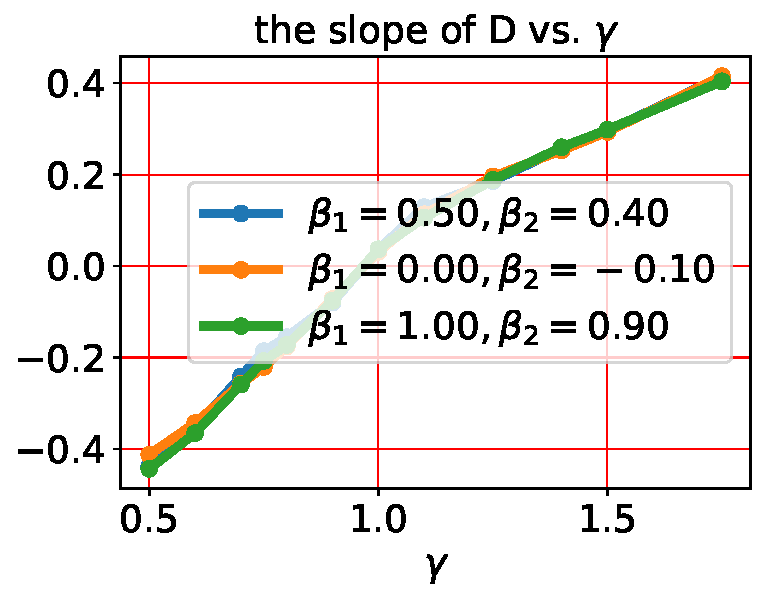
\includegraphics[scale=0.4]{pic/systemexp/gamman0.1/Dslope.pdf}
                \par\end{centering}
        }\subfloat[${\rm Cdn}$]{\begin{centering}
                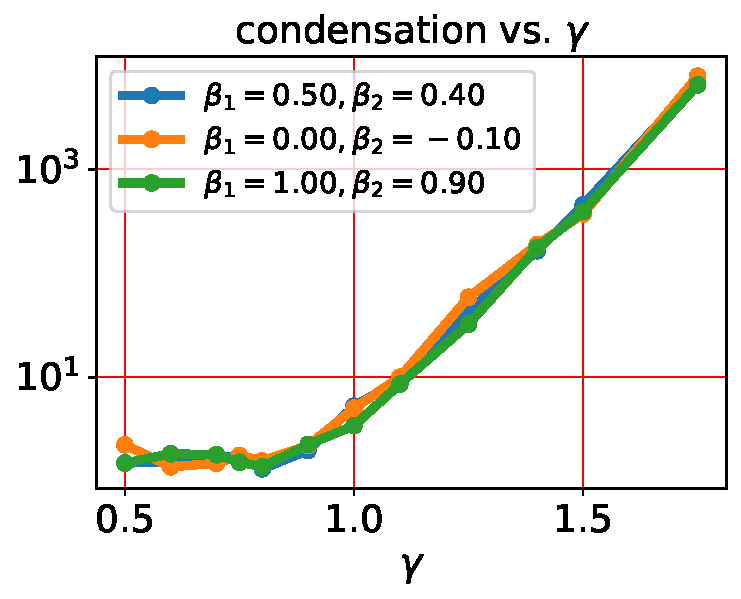
\includegraphics[scale=0.4]{pic/systemexp/gamman0.1/onesparsity-n10000.pdf}
                \par\end{centering}
        }
        \par\end{centering}
    \caption{$\gamma^{\prime}=0.1$. For (a), the slope is estimated based on NNs of $1000,5000,10000,20000,40000$ neurons. For (b) ${\rm Cdn}$ is estimated of NN of 10000 neurons for different $\alpha$. \label{fig:diffbeta} }
\end{figure}

\subsection{$\theta$-Lazy training}
In this subsection, we would empirically identify a regime where all parameters are close to their initialization after training. The slope $D_s$ is estimated based on NNs of $10^3,10^4,10^5,10^6$ neurons. Note that some experiments of $10^6$ are too slow to converge, thus, we only use other three NNs. A key point is to find a boundary where the slope transit from negative to positive. As shown in Fig. \ref{fig:ds}, we found the boundary is $\gamma=1$ regardless of $\gamma^{\prime}$.  The boundary of $\gamma=1$ indicates two folds: when $\gamma<1$, the deviation of parameters from initialization decays as neuron number increases, such as the NTK ($\gamma=0.5$, $\gamma^{\prime}=0$) studied in \cite{jacot_neural_2018}; when $\gamma\geq1$,  the deviation of parameters from initialization either increases or stay at $O(1)$ as neuron number increases, such as the mean field regime  ($\gamma=1$, $\gamma^{\prime}=0$) studied in \cite{mei_mean_2018}.

Next, we study the condensation for different pairs of $\gamma$ and $\gamma^{\prime}$.  When the condensation index is around $1$, the impact of neurons with different orientations to the NN output is similar. On the contrary, if the condensation index is very large, the NN output are dominated by neurons with some specific orientations.  As an example of $m=10^4$ shown in Fig. \ref{fig:cdn}, we similar observe that around $\gamma=1$, the condensation indexes transit from $1$ to large values, regardless of $\gamma^{\prime}$. To show the transition happen at $\gamma=1$ as neuron number increases, we study the trend of condensation index w.r.t. neuron number. For the case of NNs with one network size, we display the scatter plot of each pair of $\gamma$ and condensation index by a distinct color in Fig. \ref{fig:cdn}. For one $\gamma$, there are multiple points due the different choices of $\gamma^{\prime}$. We average condensation index over different $\gamma^{\prime}$ for each $\gamma$ and connect them by a solid color with the same color. When $\gamma<1$, the condensation index monotonically decreases with neuron number $m$. Therefore, in this regime, in the under-parameterized regime, the condensation is more significant. For example of Xavier initialization with no pre-factor ($\gamma=0.5$, $\gamma^{\prime}=-0.5$), \cite{ma2020quenching}  empirically show the transition from significant condensation to no condensation when the NN transits from the under-parameterized regime to the over-parameterized regime. On the contrary, when $\gamma>1$, the condensation index monotonically increases with neuron number. In this regime $\gamma\geq1$, as $m\rightarrow\infty$, only neurons with a few orientations are active after training. The study in \cite{maennel2018gradient} is a specific example of  $\gamma\rightarrow\infty$, where \cite{maennel2018gradient} shows that the orientations are quantized when the initial parameters approach zero.


The relative norm and the condensation of the rescaled parameters consistently classify two distinct regimes:
\begin{itemize}
    \item[1] \textbf{$\theta$-lazy regime ($\gamma<1$)}: the relative norm of $\vtheta$ decreases and condensation disappears with neuron number;
    \item[2] \textbf{Non $\theta$-lazy regime ($\gamma\geq1$)}: the relative norm of $\vtheta$ increases and  condensation amplifies with neuron number.
\end{itemize}

In the $\theta$-lazy regime, both $a$ and $\vw$ are also close to their initialization, respectively. However, in the non $\theta$-lazy regime, we would show there are different subregimes classified by the deviation from the initialization of different components in $\vtheta$ and different condensations.

BRIEFLY TALK ABOUT why THERE ARE TWO REGIMES. AND REFER TO THE THEORETICAL STUDY.

\begin{figure}
    \begin{centering}
        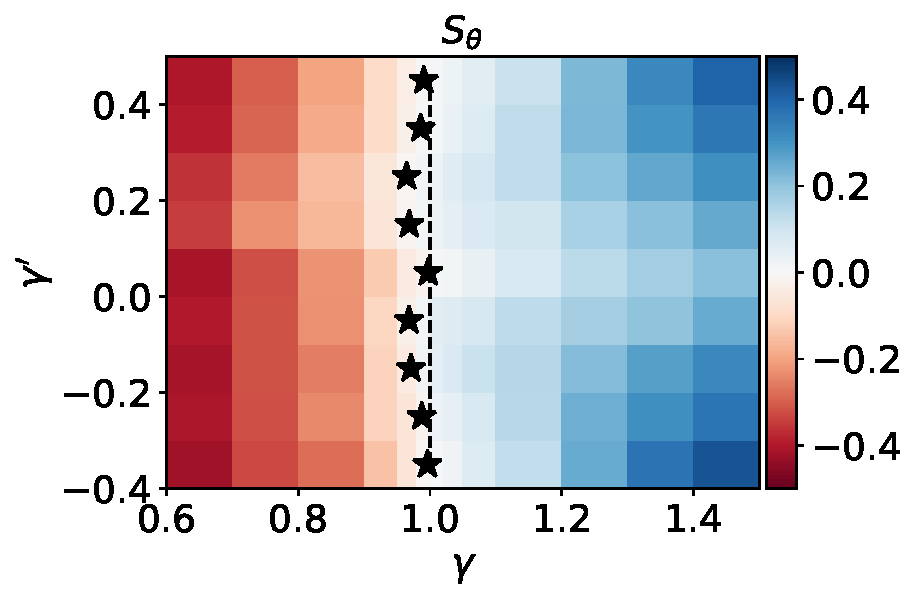
\includegraphics[scale=0.4]{pic/systemexplarg3/scalestudy3/relameansysDrescaleslope.pdf}
        \par\end{centering}
    \caption{$D_{s}$.\label{fig:ds} }
\end{figure}


\begin{figure}
    \begin{centering}
        \subfloat[$m=10000$]{\begin{centering}
                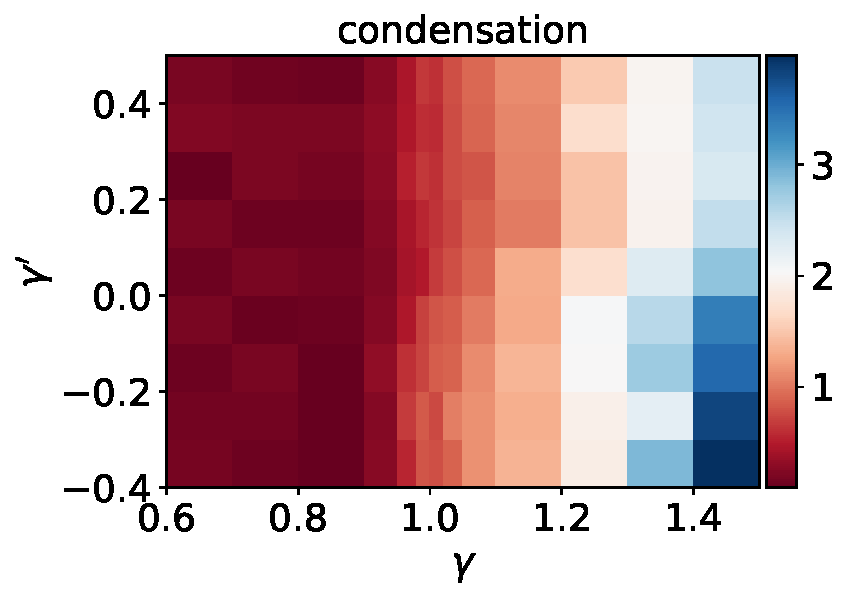
\includegraphics[scale=0.4]{pic/systemexplarg3/scalestudy3/sparsitymap_n100000.pdf}
                \par\end{centering}
        }\subfloat[${\rm Cdn}$]{\begin{centering}
                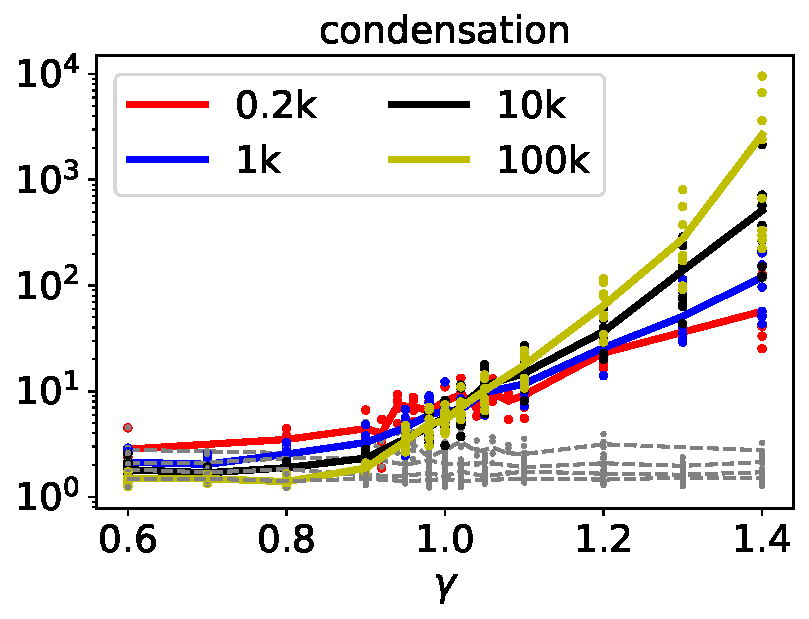
\includegraphics[scale=0.4]{pic/systemexplarg3/scalestudy3/sparsity1d.pdf}
                \par\end{centering}
        }
        \par\end{centering}
    \caption{Condensation map\label{fig:cdn} }
\end{figure}

\subsection{$a$-lazy and $w$-lazy regimes}

In the non $\theta$-lazy regime, i.e., $\gamma\geq1$, either for $a$ or $\vw$, there are also two distinct regimes. Similarly, we consider the relative distance of $(a_1, a_1, \cdots, a_m)$ and $(\vw_1, \vw_1, \cdots, \vw_m)$ from initialization.  As shown in Fig. \ref{fig:awmap}(a), for parameter $a$, the non $\theta$-lazy regime is separated by $\gamma+\gamma^{\prime}=1$. In the lower regime ($\gamma+\gamma^{\prime}<1$ and $\gamma>1$), the deviation of $a$ from initialization decays as the neuron number increases, this is $a$-lazy regime. Similarly, for parameter $\vw$, the non $\theta$-lazy regime is separated by $\gamma-\gamma^{\prime}=1$,  as shown in Fig. \ref{fig:awmap}(b). In the upper regime ($\gamma-\gamma^{\prime}>1$ and $\gamma>1$), the deviation of $\vw$ from initialization decays as the neuron number increases, that is,  $\vw$-lazy regime.

An intuitive understanding of  $a$-lazy regime and  $\vw$-lazy regime is as follows. The dynamics speed of $a$ is determined by $\vw$ and the dynamics speed of  $\vw$ is determined by $a$. When $\gamma^{\prime}$ is large, $\vw$ is initialized by a large value, thus, $a$ is trained fast. To fit the data, as the $\theta$-lazy regime indicates, $\alpha a ||\vw||_{2}$ should be larger than $O(1/m)$ after training. Consider $\gamma^{\prime}>0$, then,
\[
    \frac{\beta_1}{\beta_2}=m^{-\gamma^{\prime}}<1,
\]
that is,
\[
    \beta_1<\beta_2.
\]
At the initialization, the evolution of $a$ is much faster than $\vw$ when $m$ is large. Before $a$ evolves to $O(\beta_2)$, for simplicity, we regard $\vw$ stays close to initialization, i.e., $O(\beta_2)$. When $a$ evolves to $O(\beta_2)$, if the network is still not able to fit the data, i.e, $\alpha a ||\vw||_{2}\sim \alpha \beta_{2}^{2})$ is no larger than $O(1/m)$, $\vw$ would also start to evolve fast and deviate from its initialization of $O(\beta_2)$. If  $\alpha a ||\vw||_{2}$ is   larger than $O(1/m)$ before $a$ evolves to $O(\beta_2)$, then, before $\vw$ start to fast evolve, the NN already has capability to fit the data, in such case, $\vw$ would stay close to the initialization. The key to find the boundary of $\vw$-lazy regime is to find where the initialization satisfies $\alpha \beta_{2}^{2}=1/m$.  Now, consider the case in line $\gamma-\gamma^{\prime}=1$ and $\gamma>1$.

\begin{align}
    \alpha a ||\vw||_{2}\sim \alpha\beta_1 \beta_2=m^{-\gamma}, \\
    \frac{\beta_1}{\beta_2}=m^{-\gamma^{\prime}}=m^{-(\gamma-1)},
\end{align}
we obtain
\[
    \alpha \beta_{2}^{2}=\frac{1}{m}.
\]
Therefore, $\gamma-\gamma^{\prime}=1$ and $\gamma>1$ is the boundary for $\vw$-lazy regime. In such regime, the NN behaves like a random feature model, thus, the training dynamics of NN is a linear dynamics w.r.t. parameters. The linear regimes contains the $\theta$-lazy regime and $\vw$-lazy regime.

We can similarly analyze the boundary for $a$-lazy regime. However, in such regime, the training dynamics is nonlinear since the non-lazy variable $\vw$ is within the non-linear activation function.

\begin{figure}
    \begin{centering}
        \subfloat[$m=10000$]{\begin{centering}
                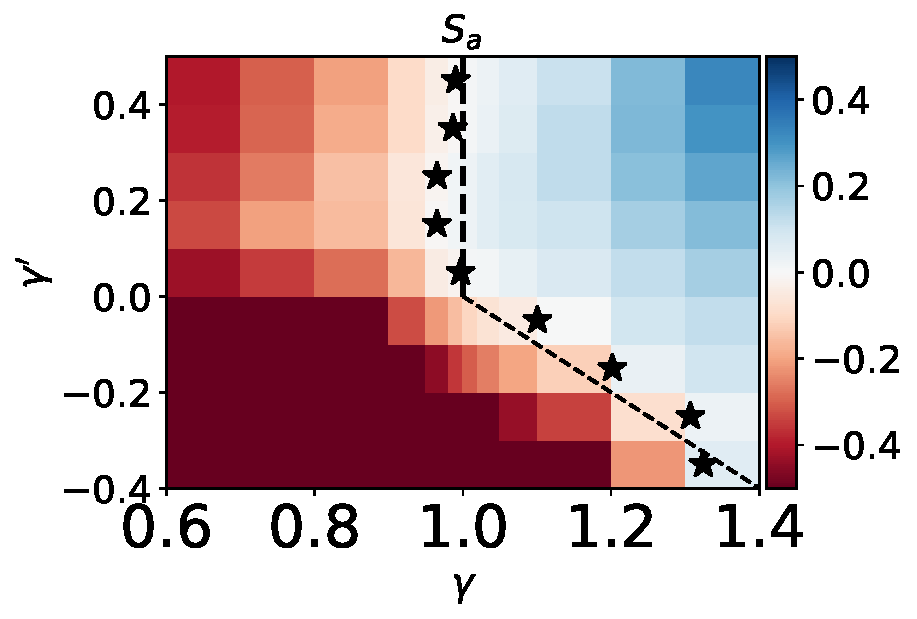
\includegraphics[scale=0.4]{pic/systemexplarg3/scalestudy3/rescale_a_slope.pdf}
                \par\end{centering}
        }\subfloat[${\rm Cdn}$]{\begin{centering}
                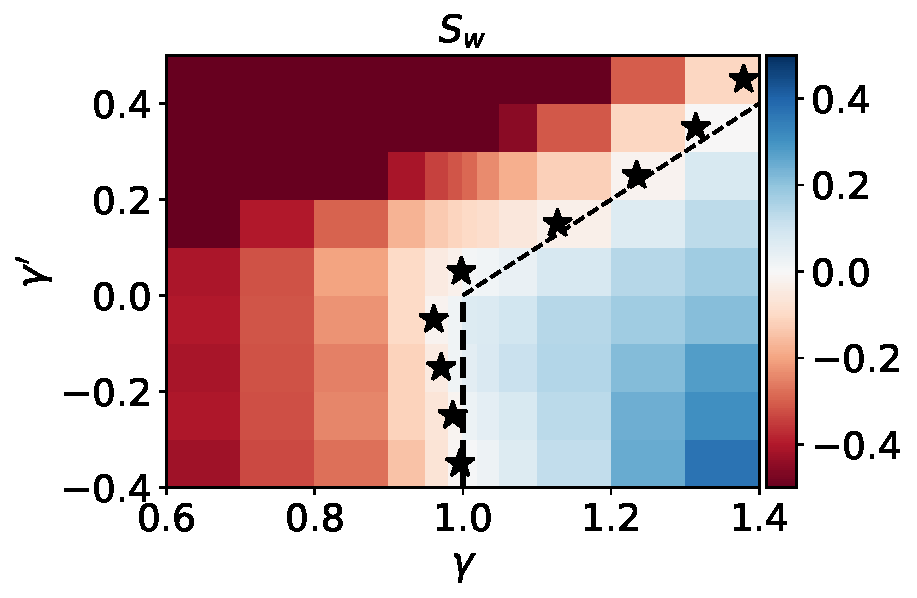
\includegraphics[scale=0.4]{pic/systemexplarg3/scalestudy3/rescale_w_slope.pdf}
                \par\end{centering}
        }
        \par\end{centering}
    \caption{input and output weight.\label{fig:awmap} }
\end{figure}


\subsection{Different condensation regime}
Neurons condense after training at the non $\theta$-lazy regime. Experiments suggest there are two different condensations illustrated as follows. For in box corresponding to a pair of $\gamma$ and $\gamma^{\prime}$, we display the absolute amplitude of each neuron versus orientation, i.e., $(|A|,\hat{\vw})$, for a network with $m$ neurons. Three networks are displayed in one box with  m=$10^{3}$ (blue), $10^{4}$ (red), $10^{6}$ (yellow), respectively. For $\gamma<1$, i.e., $\theta$-lazy regime, almost no condensation emerges, consistent with previous analysis by condensation index. For $\gamma\geq1$, the condensation has two distinct phenomena as neuron number increases separated by $\gamma-\gamma^{\prime}=1$ and $\gamma>1$ (blue boxes), which is the same boundary as the one for $\vw$-lazy training. In the upper regime ($\gamma-\gamma^{\prime}\geq1$ and $\gamma\leq1$), the width of the orientation peak stays the same as neuron number varies, while in the lower regime ($\gamma-\gamma^{\prime}>1$ and $\gamma\leq1$), the width of the orientation peak shrinks as neuron number increases.

BRIEFLY talk about why there two condensations.


\begin{figure}
    \begin{centering}
        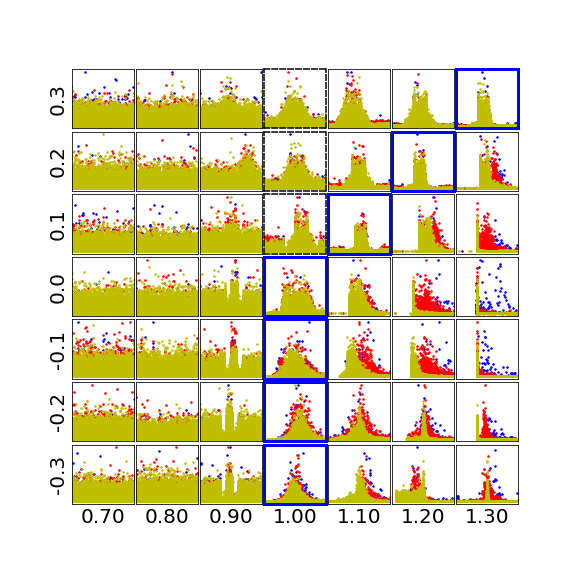
\includegraphics[scale=0.8]{pic/systemexplarg3/scalestudy3/angleamptogether.png}
        \par\end{centering}
    \caption{Condensation distribution map. The abscissa coordinate is $\gamma$ and the ordinate one is $\gamma^{\prime}$. m=$10^{3}$ (blue), $10^{4}$ (red), $10^{6}$ (yellow).\label{fig:cdnmap} }
\end{figure}

\section{Scaling Analysis and Nondimensionalization}
Similitude is a concept applicable to the testing of engineering models.


Given a sample set $S=\{(\vx_i,y_i)\}_{i=1}^n$ where $\vx_i\in\sR^d$, $i\in[n]$, network width $m$ and a scaling parameter $\alpha$ and $\sigma=\ReLU$, we define the two-layer neuron network and the empirical risk as follows
\begin{align}
    f_{\vtheta}(\vx)
     & := \alpha\sum_{j=1}^{m}a_j\sigma(\vw_j^\T\vx+b_j),                                            \\
    \RS(\vtheta)
     & :=\frac{1}{2n}\sum_{i=1}^n(f_{\vtheta}^\alpha(\vx_i)-y_i)^2                                   \\
     & =\frac{1}{2n}\sum_{i=1}^n\left(\alpha\sum_{j=1}^{m}a_j\sigma(\vw_j^\T\vx_i+b_j)-y_i\right)^2.
\end{align}
Let $\vtheta$ be the solution to the gradient flow
\begin{equation}
    \frac{\D \vtheta}{\D t}=-\nabla_{\vtheta}\RS(\vtheta).
\end{equation}
More precisely, $\vtheta=\mathrm{vec}(\vq_1,\ldots,\vq_m)$ with $\vq_j=(a_j,\vw_j^{\T},b_j)^\T$, $j\in[m]$ solves
\begin{align*}
    \frac{\D a_j}{\D t}
     & = -\frac{1}{n}\sum_{i=1}^n\alpha\sigma(\vw_j^{\T}\vx_i+b_j) \left(\alpha\sum_{j=1}^{m}a_j\sigma(\vw_j^{\T}\vx_i+b_j)-y_i\right)           \\
    \frac{\D \vw_j}{\D t}
     & = -\frac{1}{n}\sum_{i=1}^n\alpha a_j\sigma'(\vw_j^{\T}\vx_i+b_j)\vx_i \left(\alpha\sum_{j=1}^{m}a_j\sigma(\vw_j^{\T}\vx_i+b_j)-y_i\right) \\
    \frac{\D b_j}{\D t}
     & = -\frac{1}{n}\sum_{i=1}^n\alpha a_j\sigma'(\vw_j^{\T}\vx_i+b_j) \left(\alpha\sum_{j=1}^{m}a_j\sigma(\vw_j^{\T}\vx_i+b_j)-y_i\right),
\end{align*}
with initial weights:
\begin{equation}
    a_j^0\sim N(0, \beta_1^2), \quad \vw_j^0\sim N(0, \beta_2^2 \mI_d), \quad b_j^0\sim N(0, \beta_2^2).
\end{equation}
Let $\bar{a}_j=\beta_1^{-1}a_j$, $\bar{\vw}_j=\beta_2^{-1}\vw_j$ and $\bar{b}_j=\beta_2^{-1}b_j$, then
\begin{align*}
    \frac{\D \bar{a}_j}{\D \bar{t}}
     & = -\frac{\beta_2}{\beta_1}\frac{1}{n}\sum_{i=1}^n \alpha\sigma(\bar{\vw}_j^\T\vx_i+\bar{b}_j) \left(\alpha\beta_1\beta_2\sum_{j=1}^{m}\bar{a}_j\sigma(\bar{\vw}_j^\T\vx_i+\bar{b}_j)-y_i\right),               \\
    \frac{\D \bar{\vw}_j}{\D \bar{t}}
     & = -\frac{\beta_1}{\beta_2}\frac{1}{n}\sum_{i=1}^n\alpha\bar{a}_j\sigma'(\bar{\vw}_j^\T\vx_i+\bar{b}_j)\vx_i \left(\alpha\beta_1\beta_2\sum_{j=1}^{m}\bar{a}_j\sigma(\bar{\vw}_j^\T\vx_i+\bar{b}_j)-y_i\right), \\
    \frac{\D \bar{b}_j}{\D \bar{t}}
     & = -\frac{\beta_1}{\beta_2}\frac{1}{n}\sum_{i=1}^n\alpha\bar{a}_j\sigma'(\bar{\vw}_j^\T\vx_i+\bar{b}_j) \left(\alpha\beta_1\beta_2\sum_{j=1}^{m}\bar{a}_j\sigma(\bar{\vw}_j^\T\vx_i+\bar{b}_j)-y_i\right).
\end{align*}
We introduce two scaling parameters, i.e., $\kappa:=\alpha\beta_1\beta_2$ (energetic scale parameter) and $\kappa':=\frac{\beta_1}{\beta_2}$ (dynamical scale parameter), then the above dynamics can be written as
\begin{align*}
    \frac{\D \bar{a}_j}{\D \bar{t}}
     & = -\frac{1}{\kappa'}\frac{1}{n}\sum_{i=1}^n \alpha\sigma(\bar{\vw}_j^\T\vx_i+\bar{b}_j) \left(\kappa\sum_{j=1}^{m}\bar{a}_j\sigma(\bar{\vw}_j^\T\vx_i+\bar{b}_j)-y_i\right),     \\
    \frac{\D \bar{\vw}_j}{\D \bar{t}}
     & = -\kappa'\frac{1}{n}\sum_{i=1}^n\alpha\bar{a}_j\sigma'(\bar{\vw}_j^\T\vx_i+\bar{b}_j)\vx_i \left(\kappa\sum_{j=1}^{m}\bar{a}_j\sigma(\bar{\vw}_j^\T\vx_i+\bar{b}_j)-y_i\right), \\
    \frac{\D \bar{b}_j}{\D \bar{t}}
     & = -\kappa'\frac{1}{n}\sum_{i=1}^n\alpha\bar{a}_j\sigma'(\bar{\vw}_j^\T\vx_i+\bar{b}_j) \left(\kappa\sum_{j=1}^{m}\bar{a}_j\sigma(\bar{\vw}_j^\T\vx_i+\bar{b}_j)-y_i\right).
\end{align*}
In the following discussion we will drop the ``bar''s of $a_j$, $\vw_j$, $b_j$ and correspondingly $\vtheta$, $\vq_j$ for simplicity. Define
\begin{align}
    f^{\kappa}_{\vtheta}(\vx)
     & := \kappa\sum_{j=1}^{m}a_j\sigma(\vw_j^\T\vx+b_j),               \\
    R_{S, \kappa}(\vtheta)
     & :=\frac{1}{2n}\sum_{i=1}^n{(f^{\kappa}_{\vtheta}(\vx_i)-y_i)}^2,
\end{align}
then the weighted GD is
\begin{equation}
    \frac{\D\vq_j}{\D t} = -\frac{\alpha}{\kappa}\mM_{\kappa'}\nabla_{\vq_j}R_{S,\kappa}(\vtheta),
\end{equation}
where the mobility matrix
\begin{equation}
    \mM_{\kappa'} = -
    \begin{pmatrix}
        \frac{1}{\kappa'} &         &         \\
                          & \kappa' &         \\
                          &         & \kappa'
    \end{pmatrix},
\end{equation}
the ``learning rate'' in practical application can be understood as $\eta = \frac{\alpha}{\kappa}$. Up to this $\eta$ we rescale the time furthermore to obtain an equivelent ``standardize'' dynamics:
\begin{equation}
    \frac{\D \vq_j}{\D t} = -\mM_{\kappa'}\nabla_{\vq_j}R_{S, \kappa}(\vtheta),
\end{equation}
more precisely
\begin{align*}
    \frac{\D a_j}{\D t}
     & = -\frac{1}{\kappa'}\frac{1}{n}\sum_{i=1}^n \kappa\sigma(\vw_j^\T\vx_i+b_j) \left(\kappa\sum_{j=1}^{m}a_j\sigma(\vw_j^\T\vx_i+b_j)-y_i\right), \\
    \frac{\D \vw_j}{\D t}
     & = -\kappa'\frac{1}{n}\sum_{i=1}^n\kappa a_j\sigma'(\vw_j^\T\vx_i+b_j)\vx_i \left(\kappa\sum_{j=1}^{m}a_j\sigma(\vw_j^\T\vx_i+b_j)-y_i\right),  \\
    \frac{\D b_j}{\D t}
     & = -\kappa'\frac{1}{n}\sum_{i=1}^n\kappa a_j\sigma'(\vw_j^\T\vx_i+b_j) \left(\kappa\sum_{j=1}^{m}a_j\sigma(\vw_j^\T\vx_i+b_j)-y_i\right),
\end{align*}
whose initials are
\begin{equation}
    a_j^0\sim N(0,1), \quad \vw_j^0\sim N(0,\mI_d), \quad b_j^0\sim N(0, 1).
\end{equation}
Furthermore, given $\kappa'$ (e.g. $\mM_{\kappa'}$) let $\tilde{a}_j = \sqrt{\kappa}a_j$, $\tilde{\vw}_j = \sqrt{\kappa}\vw_j$, $\tilde{b}_j=\sqrt{\kappa}b_j$ and $\tilde{t}=\kappa t$ then
\begin{align*}
    \frac{\D \tilde{a}_j}{\D \tilde{t}}
     & = -\frac{1}{\kappa'}\frac{1}{n}\sum_{i=1}^n\sigma(\tilde{\vw}_j^\T\vx_i+\tilde{b}_j) \left(\sum_{j=1}^{m}\tilde{a}_j\sigma(\tilde{\vw}_j^\T\vx_i+\tilde{b}_j)-y_i\right),        \\
    \frac{\D \tilde{\vw}_j}{\D \tilde{t}}
     & = -\kappa'\frac{1}{n}\sum_{i=1}^n\tilde{a}_j\sigma'(\tilde{\vw}_j^\T\vx_i+\tilde{b}_j)\vx_i \left(\sum_{j=1}^{m}\tilde{a}_j\sigma(\tilde{\vw}_j^\T\vx_i+\tilde{b}_j)-y_i\right), \\
    \frac{\D \tilde{b}_j}{\D \tilde{t}}
     & = -\kappa'\frac{1}{n}\sum_{i=1}^n\tilde{a}_j\sigma'(\tilde{\vw}_j^\T\vx_i+\tilde{b}_j) \left(\sum_{j=1}^{m}\tilde{a}_j\sigma(\tilde{\vw}_j^\T\vx_i+\tilde{b}_j)-y_i\right),
\end{align*}
where
\begin{equation}
    \tilde{a}^0_j\sim N(0, \kappa), \quad \tilde{\vw}_j^0\sim N(0, \kappa\mI_d), \quad \tilde{b}^0_j\sim N(0, \kappa).
\end{equation}
$\tilde{\vtheta}$ follows the weighted GD of
\begin{align}
    f_{\tilde{\vtheta}}(\vx)
     & := \sum_{j=1}^{m}\tilde{a}_j\sigma(\tilde{\vw}_j^\T\tilde{\vx}+\tilde{b}_j), \\
    \RS(\tilde{\vtheta})
     & :=\frac{1}{2n}\sum_{i=1}^n(f_{\tilde{\vtheta}}^\alpha(\vx_i)-y_i)^2.
\end{align}
that is,
\begin{equation}
    \frac{\D \tilde{\vtheta}}{\D\tilde{t}} = -\mM_{\kappa'}\nabla_{\tilde{\vtheta}}\RS(\tilde{\vtheta})
\end{equation}
Note that $\tilde{\vtheta}(+\infty)=\sqrt{\kappa}\vtheta(+\infty)$ given $\tilde{\vtheta}^0=\sqrt{\kappa}\vtheta^0$. Let $M=m(d+2)$ and $\vTheta:\sR^+\times\sR^M\to\sR^M$ be a flow satisfying
\begin{align}
    \vTheta(0,\vtheta)
     & = \vtheta,              \\
    \vTheta(s,\vTheta(t,\vtheta))
     & = \vTheta(s+t,\vtheta).
\end{align}
In particular, we define $\vTheta(t,\vtheta^0)=\vtheta(t)$ with $\vtheta(0)=\vtheta^0$ and $\tilde{\vTheta}(t,\vtheta^0)=\tilde{\vtheta}(t)$ with $\tilde{\vtheta}(0)=\tilde{\vtheta}^0$.

\section{Regimes characterization}

Now we consider the dynamics of $\tilde{\vtheta}$ by dropping ``\textasciitilde{}'' for simplicity then the two layer neural network is
\begin{equation}
    f_{\vtheta}(\vx) = \sum_{k=1}^{m} a_k\sigma(\vw_k\cdot\vx),
\end{equation}
with activation function $\sigma(z) = \ReLU(z) = \max(z, 0)$. Denote the dataset
\begin{equation}
    S = {\{(\vx_i, y_i)\}}_{i=1}^n \sim \fD(\Omega),
\end{equation}
where $\vx_i$ are i.i.d.\ sampled from distribution $\fD$ over $\Omega={[0,1]}^d$ and $(\vx_i)_d=1$ such that $\norm{\vx_i}_2\leq\sqrt{d}$ and $y_i=f(\vx_i)\in[0,1]$ for all $i$.

We denote $e_i = f_{\vtheta}(\vx_i) - y_i = f_{\vtheta}(\vx_i) - f(\vx_i)$ and $\ve = {(e_1, e_2, \ldots, e_n)}^{\T}$ then the empirical risk can be written as
\begin{equation}
    \RS(\vtheta) = \frac{1}{2n}\sum_{i=1}^n{\left(f_{\vtheta}(\vx_i)-y_i\right)}^2 = \frac{1}{2n}\ve^{\T}\ve.
\end{equation}
The gradient descent (GD) dynamics is
\begin{equation}\label{eqn:gd_dyn}
    \dot{\vtheta} = -M_{\kappa'}\nabla_{\vtheta}\RS(\vtheta),
\end{equation}
with a more explicit form for $a_k$ and $\vw_k$ respectively
\begin{equation}
    \left \{
    \begin{aligned}
        \dot{a}_k   & = -\frac{1}{\kappa'}\nabla_{a_k}\RS(\vtheta) = -\frac{1}{\kappa'n}\sum_{i=1}^{n}e_i\sigma(\vw_k\cdot\vx_i), \\
        \dot{\vw}_k & =-\kappa'\nabla_{\vw_k}\RS(\vtheta) = -\frac{\kappa'}{n}\sum_{i=1}^n e_i a_i\sigma'(\vw_k\cdot\vx_i)\vx_i.
    \end{aligned}
    \right.
\end{equation}
The initialization of parameters are
\begin{align}
     & a^0_k:=a_k(0)\sim N(0,\kappa),\quad\text{then }\bar{a}_k^0:=\bar{a}_k(0)=\frac{1}{\sqrt{\kappa}}a_k(0)\sim N(0,1)                     \\
     & \vw_k^0:=\vw_k(0)\sim N(0, \kappa\mI_d),\quad\text{then }\bar{\vw}_k^0:=\bar{\vw}_k(0)=\frac{1}{\sqrt{\kappa}}\vw_k(0)\sim N(0,\mI_d) \\
     & \vtheta^0 = \vtheta(0) = {\{(a_k^0, \vw_k^0)\}}_{k=1}^m, \quad\text{then }\bar{\vtheta}^0=\bar{\vtheta}(0).
\end{align}
The kernels of the GD dynamics are
\begin{equation}
    \begin{aligned}
         & \mK^{(a)}(\vx,\vx')=\Exp_{\bar{\vw}}\sigma(\bar{\vw}\cdot\vx)\sigma(\bar{\vw}\cdot\vx'),                                    \\
         & \mK^{(\vw)}(\vx,\vx')=\Exp_{(\bar{a},\bar{\vw})}\bar{a}^2\sigma'(\bar{\vw}\cdot\vx)\sigma'(\bar{\vw}\cdot\vx')\vx\cdot\vx'. \\
    \end{aligned}
\end{equation}
The Gram maxtrices of infinite width are
\begin{equation}
    \begin{aligned}
         & K^{(a)}_{ij}=\mK^{(a)}(\vx_i,\vx_j), \quad \mK^{(a)}=(K_{ij}^{(a)})_{n\times n},         \\
         & K^{(\vw)}_{ij}=\mK^{(\vw)}(\vx_i,\vx_j), \quad \mK^{(\vw)}=(K_{ij}^{(\vw)})_{n\times n}.
    \end{aligned}
\end{equation}

\noindent The Gram matrices $\mG^{(a)},\mG^{(\vw)}$ and $\mG$ of finite width have the following expressions
\begin{equation}
    \begin{aligned}
         & G^{(a)}_{ij}(\vtheta)=\frac{1}{\kappa' m}\sum_{k=1}^m\sigma(\vw_k\cdot\vx_i)\sigma(\vw_k\cdot\vx_j),                        \\
         & G^{(\vw)}_{ij}(\vtheta)=\frac{\kappa'}{m}\sum_{k=1}^m a_k^2\sigma'(\vw_k\cdot\vx_i)\sigma'(\vw_k\cdot\vx_j)\vx_i\cdot\vx_j, \\
         & \mG=\mG^{(a)}+\mG^{(\vw)}.
    \end{aligned}
\end{equation}
\begin{assump}\label{assump:main}
    We assume that
    \begin{equation}
        \lambda_S^{(a)} := \lambda_{\min}\left(\mK^{(a)}\right) > 0,\quad \lambda_S^{(\vw)} := \lambda_{\min}\left(\mK^{(\vw)}\right) > 0,
    \end{equation}
    and denote
    \begin{equation}
        \lambda_S:=\min \{\lambda_S^{(a)},\lambda_S^{(\vw)}\}\leq d.
    \end{equation}
\end{assump}
\begin{rmk}
    We expect that:
    \begin{equation}
        \begin{aligned}
            \mG^{(a)}(\vtheta^0)   & \approx\frac{\kappa}{\kappa'}\mK^{(a)}, \\
            \mG^{(\vw)}(\vtheta^0) & \approx\kappa\kappa'\mK^{(\vw)},
        \end{aligned}
    \end{equation}
    and this will be rigorously achieved in the following proofs.
\end{rmk}
In the following discussion, we consider the following quantities
\begin{equation}
    \alpha(t)=\max\limits_{k\in[m],s\in[0,t]}|a_k(s)|, \quad \omega(t)=\max\limits_{k\in[m],s\in[0,t]}\norm{\vw_k(s)}_{\infty},
\end{equation}
which is convenient for our technical proof.
\begin{lem}\label{lem1}
    For any $\delta\in(0,1)$ with probability at least $1-\delta$ over initialization, we have
    \begin{equation}\label{eqn:lem1}
        \max\limits_{k\in[m]}\left\{\abs{a_k^0},\;\norm{\vw_k^0}_{\infty}\right \}\leq\sqrt{\kappa}\sqrt{2\log\frac{2m(d+1)}{\delta}},
    \end{equation}
\end{lem}
\begin{proof}
    If $\rX \sim N(0, 1)$, then $\Prob(\abs{\rX} > \eps) \leq 2\E^{-\frac{1}{2}\eps^2}$ for all $\eps > 0$. Since $\bar{a}^0_k\sim N(0,1)$, ${(\bar{w}_k^0)}_{\alpha}\sim N(0,1)$ for $k=1, 2, \ldots, m,\; \alpha =1,\ldots,d$ and they are all independent, by setting
    \begin{equation}
        \eps = \sqrt{2\log\frac{2m(d+1)}{\delta}},
    \end{equation}
    one can obtain
    \begin{equation}
        \begin{aligned}
            \Prob\left(\max\limits_{k\in[m]}\left\{\abs{\bar{a}_k^0},\; \norm{\bar{\vw}_k^0}_{\infty}\right \}>\eps\right)
             & = \Prob\left(\max\limits_{k\in[m],\alpha\in[d]}\left\{\abs{\bar{a}_k^0},\; \abs{{(\bar{w}^0_k)}_{\alpha}}\right \}>\eps\right)                                            \\
             & = \Prob\left(\bigcup\limits_{k=1}^m\left(\abs{\bar{a}_k^0}>\eps\right)\cup\left(\bigcup\limits_{\alpha=1}^d\left(\abs{{(\bar{w}_k^0)}_{\alpha}}>\eps\right)\right)\right) \\
             & \leq \sum_{k=1}^m \Prob\left(\abs{\bar{a}_k^0}>\eps\right) + \sum_{k=1}^m\sum_{\alpha=1}^d \Prob\left(\abs{{(\bar{w}^0_k)}_{\alpha}}>\eps\right)                          \\
             & \leq 2m \E^{-\frac{1}{2}\eps^2} + 2md \E^{-\frac{1}{2}\eps^2}                                                                                                             \\
             & = 2m(d+1)\E^{-\frac{1}{2}\eps^2}                                                                                                                                          \\
             & = \delta.
        \end{aligned}
    \end{equation}
\end{proof}
\begin{lem}
    For any $\delta\in(0,1)$ with probability at least $1-\delta$ over initialization, we have
    \begin{equation}
        \RS(\vtheta^0)\leq\frac{1}{2}\left[1 + 2d\left(\log\frac{4m(d+1)}{\delta}\right)\left(2+3\sqrt{2\log(8/\delta)}\right)\kappa\sqrt{m}\right]^2.
    \end{equation}
\end{lem}
\begin{proof}
    From Lemma~\ref{lem1} we know that with probability at least $1-\delta/2$,
    \begin{equation}
        \abs{\bar{a}_k^0} \leq \sqrt{2\log\frac{4m(d+1)}{\delta}} \quad \text{and} \quad \norm{\bar{\vw}_k^0}_2 \leq \sqrt{2d\log\frac{4m(d+1)}{\delta}}.
    \end{equation}
    Let
    \begin{equation}
        \fF = \{g(\bar{a},\bar{\vw}) \mid g(\bar{a},\bar{\vw}):=\bar{a}\sigma(\bar{\vw}\cdot\vx),\vx\in\Omega \},
    \end{equation}
    then with prob$\geq 1-\delta/2$
    \begin{equation}
        \abs{g(\bar{a}^0_k,\bar{\vw}^0_k)}\leq\sqrt{d}\sqrt{2\log\frac{4m(d+1)}{\delta}}\sqrt{2d\log\frac{4m(d+1)}{\delta}}=2d\log\frac{4m(d+1)}{\delta}
    \end{equation}
    Then
    \begin{equation}
        \begin{aligned}
            \frac{1}{\kappa m}\sup_{\vx\in\Omega}\abs{f_{\vtheta^0}(\vx)}
             & =\sup_{\vx\in\Omega}\left\lvert \frac{1}{m}\sum_{k=1}^m \bar{a}_k^0\sigma(\bar{\vw}_k^0\cdot\vx)-\Exp_{(\bar{a},\bar{\vw})}\bar{a}\sigma(\bar{\vw}\cdot\vx)\right\rvert \\
             & \leq 2\Rad_{\bar{\vtheta}^0}(\fF) + 6d \left(\log\frac{4m(d+1)}{\delta}\right)\sqrt{\frac{2\log(8/\delta)}{m}}.
        \end{aligned}
    \end{equation}
    The Rademacher complexity can be computed assume
    \begin{equation}
        \begin{aligned}
            \Rad_{\bar{\vtheta}^0}(\fF)
             & =\frac{1}{m}\Exp_{\tau}\left[\sup_{\vx\in\Omega}\sum_{k=1}^m\tau_k\bar{a}^0_k\sigma(\bar{\vw^0_k\cdot\vx})\right]                   \\
             & \leq\frac{1}{m}\sqrt{2\log\frac{4m(d+1)}{\delta}}\Exp_{\tau}\left[\sup_{\vx\in\Omega}\sum_{k=1}^m\tau_k\bar{\vw}^0_k\cdot\vx\right] \\
             & \leq\sqrt{2\log\frac{4m(d+1)}{\delta}}\sqrt{2d\log\frac{4m(d+1)}{\delta}}\frac{\sqrt{d}}{\sqrt{m}}                                  \\
             & =\frac{2d\log\frac{4m(d+1)}{\delta}}{\sqrt{m}}.
        \end{aligned}
    \end{equation}
    So
    \begin{equation}
        \sup_{\vx\in\Omega}\abs{f_{\vtheta^0}(\vx)}\leq 2d\left(\log\frac{4m(d+1)}{\delta}\right)(2+3\sqrt{2\log(8/\delta)}\kappa\sqrt{m}),
    \end{equation}
    and
    \begin{equation}
        \begin{aligned}
            \RS(\vtheta^0)
             & \leq\frac{1}{2n}\sum_{i=1}^n{\left(1+\abs{f_{\vtheta}(\vx_i)}\right)}^2                                                          \\
             & \leq\frac{1}{2}{\left[1+2d\left(\log\frac{4m(d+1)}{\delta}\right)\left(2+3\sqrt{2\log(8/\delta)}\kappa\sqrt{m}\right)\right]}^2.
        \end{aligned}
    \end{equation}
\end{proof}
\begin{rmk}
    If $\kappa=O(\frac{1}{\sqrt{m}\log m})$ then $\RS(\vtheta^0)=O(1)$. One can use ASI trick to guarantee $\RS(\vtheta^0)\leq\frac{1}{2}$ for any $\kappa$.
\end{rmk}
\begin{defi}[Sub-expenential norm]
    If $\rX$ is a random variable, we define the sub-expenential norm as
    \begin{equation}
        \norm{\rX}_{\psi_1} := \inf\{s>0 \mid \Exp[e^{\frac{\abs{\rX}}{s}}]\leq 2\},
    \end{equation}
    and we let $C_{\psi,d}:=\left\lVert\norm{\vw}_2^2\right\rVert_{\psi_1} = \norm{\chi^2(d)}_{\psi_1}$ where $\vw\sim N(0,\mI_d)$ and $\chi^2(d)$ is $\chi^2$ distribution with $d$ degrees of freedom whose probability density function is
    \begin{equation}
        f_z(z)=\frac{1}{2^{d/2}\Gamma(d/2)}z^{d/2-1}e^{-z/2}.
    \end{equation}
\end{defi}
\begin{rmk}
    We remark that by above definition $C_{\psi,d}<+\infty$ and $\Exp_{z\sim\chi^2(d)}e^{\abs{z}/2}=+\infty$ implies $C_{\psi,d}\geq 2$.
\end{rmk}
\begin{rmk}
    Suppose that $\vw\sim N(0,\mI_d)$, $a\sim N(0,1)$ and given $\vx_i,\vx_j \in\Omega$,
    \begin{enumerate}
        \item consider $\rX:=\sigma(\vw\cdot\vx_i)\sigma(\vx\cdot\vx_j)$ and $\rZ:=\norm{\vw}^2_2=\chi^2(d)$, then $\abs{\rX}\leq d\norm{\vw}^2_2=d\rZ$ and
              \begin{equation}
                  \begin{aligned}
                      \norm{\rX}_{\phi_1}
                       & =\inf\{s>0\mid\Exp_{\rX}\exp(\abs{\rX}/s)\leq 2\}                                                   \\
                       & =\inf\{s>0\mid\Exp_{\vw}\exp\left(\abs{\sigma(\vw\cdot\vx_i)\sigma(\vw\cdot\vx_j)}/s\right)\leq 2\} \\
                       & \leq\inf\{s>0\mid\Exp_{\vw}\exp(d\norm{\vw}^2_2/s)\leq 2\}                                          \\
                       & =\inf\{s>0\mid\Exp_{\rZ}\exp(d\abs{rZ}/s)\leq 2\}                                                   \\
                       & =d\inf\{s>0\mid\Exp_{\rZ}\exp(\abs{\rZ}/s)\leq 2\}                                                  \\
                       & =d\norm{\chi^2(d)}_{\psi_1}                                                                         \\
                       & \leq dC_{\psi,d}.
                  \end{aligned}
              \end{equation}
        \item consider $\rX:=a^2\sigma'(\vw\cdot\vx_i)\sigma'(\vw\cdot\vx_j)\vx_i\cdot\vx_j$ then $\abs{\rX}\leq d\abs{a}^2\leq d\rZ$ and $\norm{\rX}_{\psi_1}\leq dC_{\psi,d}$.
    \end{enumerate}
\end{rmk}
\begin{thm}[Sub-expenential Bernstein's inequality]\label{thm:sub_exp}
    Suppose $\rX_1,\ldots,\rX_m$ are i.i.d. sub-expenential random variables with $\Exp\rX_1=\mu$, then $\forall s\geq 0$ we have
    \begin{equation}
        \Prob\left(\abs{\frac{1}{m}\sum_{k=1}^m\rX_k-\mu}\geq s\right)\leq 2\exp\left(-C_0 m \min\left(\frac{s^2}{\norm{\rX_1}^2_{\psi_1}},\frac{s}{\norm{\rX_1}_{\psi_1}}\right)\right),
    \end{equation}
    where $C_0$ is an absolute constant.
\end{thm}
\begin{lem}\label{lem:lambda_min}
    For any $\delta\in(0,1)$ if $m\geq\frac{16n^2d^2C_{\psi,d}}{C_0\lambda_S^2}\log\frac{4n^2}{\delta}$ then with probability at least $1-\delta$ over initialization, we have
    \begin{equation}
        \lambda_{\min}\left(\mG(\vtheta^0)\right)\geq\frac{3}{4}\left(\frac{\kappa}{\kappa'}\lambda_S^{(a)}+\kappa\kappa'\lambda_S^{(\vw)}\right).
    \end{equation}
\end{lem}
\begin{proof}
    $\forall \eps > 0$, we define
    \begin{equation}
        \begin{aligned}
            \Omega_{ij}^{(a)}   & :=\left\{\vtheta^0 \mid \left\lvert \frac{\kappa'}{\kappa}G^{(a)}_{ij}(\vtheta^0) - K^{(a)}_{ij}\right\rvert \leq \frac{\eps}{n} \right\}        \\
            \Omega_{ij}^{(\vw)} & := \left\{\vtheta^0 \mid \left\lvert \frac{1}{\kappa\kappa'}G^{(\vw)}_{ij}(\vtheta^0) - K^{(\vw)}_{ij}\right\rvert \leq \frac{\eps}{n} \right\}.
        \end{aligned}
    \end{equation}
    Then from Theorem~\ref{thm:sub_exp} and Remark~\ref{lem:lambda_min} we know if $\frac{\eps}{ndC_{\psi,d}}\leq 1$ then
    \begin{equation}
        \begin{aligned}
            \Prob(\Omega^{(a)}_{ij})   & \geq 1-2\exp\left(-\frac{mC_0\eps^2}{n^2d^2C_{\psi,d}^2}\right), \\
            \Prob(\Omega^{(\vw)}_{ij}) & \geq 1-2\exp\left(-\frac{mC_0\eps^2}{n^2d^2C_{\psi,d}^2}\right),
        \end{aligned}
    \end{equation}
    so with $\mathrm{prob}\geq \left[1-2\exp\left(-\frac{mC_0\eps^2}{n^2d^2C_{\psi,d}^2}\right)\right]^{2n^2} \geq 1-4n^2\exp\left(-\frac{mC_0\eps^2}{n^2d^2C_{\psi,d}^2}\right)$, we have
    \begin{equation}
        \begin{aligned}
             & \norm{\frac{\kappa'}{\kappa}\mG^{(a)}(\vtheta^0) - \mK^{(a)}}_F \leq \eps,      \\
             & \norm{\frac{1}{\kappa\kappa'}\mG^{(\vw)}(\vtheta^0) - \mK^{(\vw)}}_F \leq \eps,
        \end{aligned}
    \end{equation}
    Hence by taking $\eps=\lambda_S/4$, that is, $\delta=4n^2\exp\left(-\frac{mC_0\lambda_S^2}{16n^2d^2C_{\psi,d}^2}\right)$
    \begin{equation}
        \begin{aligned}
            \lambda_{\min}\left(\mG(\vtheta^0)\right)
             & \geq\lambda_{\min}\left(\mG^{(a)}(\vtheta^0)\right) + \lambda_{\min}\left(\mG^{(\vw)}(\vtheta^0)\right)                          \\
             & \geq\frac{\kappa}{\kappa'}\lambda_S^{(a)}-\frac{\kappa}{\kappa'} \norm{\frac{\kappa'}{\kappa}\mG^{(a)}(\vtheta^0) - \mK^{(a)}}_F \\
             & \quad + \kappa\kappa'\lambda_S^{(\vw)} - \kappa\kappa'\norm{\frac{1}{\kappa\kappa'}\mG^{(\vw)}(\vtheta^0) - \mK^{(\vw)}}_F       \\
             & \geq\frac{\kappa}{\kappa'}(\lambda_S^{(a)}-\eps)+\kappa\kappa'(\lambda_S^{(\vw)}-\eps)                                           \\
             & \geq\frac{3}{4}\left(\frac{\kappa}{\kappa'}\lambda_S^{(a)}+\kappa\kappa'\lambda_S^{(\vw)}\right).
        \end{aligned}
    \end{equation}
\end{proof}

\noindent In the following we denote
\begin{equation}
    t^* = \inf\{t \mid \vtheta(t)\notin \mathcal{N}(\vtheta^0)\},
\end{equation}
where
\begin{equation}
    \mathcal{N}(\vtheta^0) := \left\{\theta \mid \norm{\mG(\vtheta) - \mG(\vtheta^0)}_F\leq \frac{1}{4}\left(\frac{\kappa}{\kappa'}\lambda_S^{(a)}+\kappa\kappa'\lambda_S^{(\vw)}\right)\right\}.
\end{equation}
Then we have the following lemma
\begin{lem}\label{lem:exp_RS}
    For any $\delta\in(0,1)$, if $m\geq\frac{16n^2d^2C_{\psi,d}^2}{\lambda_S^2C_0}\log\frac{4n^2}{\delta}$, then with probability at least $1-\delta$ over initialization, we have for any $t\in[0, t^*)$
    \begin{equation}
        \RS(\vtheta(t)) \leq \exp\left(-\frac{m}{n}\left(\frac{\kappa}{\kappa'}\lambda_S^{(a)}+\kappa\kappa'\lambda_S^{(\vw)}\right)\right)\RS(\vtheta^0).
    \end{equation}
\end{lem}
\begin{proof}
    From Lemma~\ref{lem:lambda_min}, for any $\delta\in(0,1)$ with probability at least $1-\delta$ and for any $\vtheta\in\mathcal{N}(\vtheta^0)$,
    \begin{equation}
        \begin{aligned}
            \lambda_{\min}\left(\mG(\vtheta)\right)
             & \geq \lambda_{\min}\left(\mG(\vtheta^0)\right) - \norm{\mG(\vtheta) - \mG(\vtheta^0)}_F                                                                                                          \\
             & \geq \frac{3}{4}\left(\frac{\kappa}{\kappa'}\lambda_S^{(a)}+\kappa\kappa'\lambda_S^{(\vw)}\right) - \frac{1}{4}\left(\frac{\kappa}{\kappa'}\lambda_S^{(a)}+\kappa\kappa'\lambda_S^{(\vw)}\right) \\
             & = \frac{1}{2}\left(\frac{\kappa}{\kappa'}\lambda_S^{(a)}+\kappa\kappa'\lambda_S^{(\vw)}\right).
        \end{aligned}
    \end{equation}
    Note that
    \begin{equation}
        G_{ij} = G_{ij}^{(a)}+G^{\vw}_{ij}=\frac{1}{m}\nabla_{a}f_{\vtheta}(\vx_i)\cdot\nabla_{a}f_{\vtheta}(\vx_j)\frac{1}{\kappa'}+\frac{1}{m}\nabla_{\vw}f_{\vtheta}(\vx_i)\cdot\nabla_{\vw}f_{\vtheta}(\vx_j)\kappa',
    \end{equation}
    and
    \begin{equation}
        \begin{aligned}
            \nabla_{a}\RS(\vtheta)   & =\frac{1}{n}\sum_{i=1}^{n}e_i\nabla_{a}f_{\vtheta}(\vx_i),    \\
            \nabla_{\vw}\RS(\vtheta) & = \frac{1}{n}\sum_{i=1}^{n}e_i\nabla_{\vw}f_{\vtheta}(\vx_i),
        \end{aligned}
    \end{equation}
    so
    \begin{equation}
        \frac{m}{n^2}\ve^{\T}\mG^{(a)}\ve=\frac{1}{\kappa'}\nabla_a\RS\cdot\nabla_{a}\RS+\kappa'\nabla_{\vw}\RS\cdot\nabla_{\vw}\RS,
    \end{equation}
    Then finally we get
    \begin{equation}
        \begin{aligned}
            \frac{\D}{\D t}\RS(\vtheta(t))
             & =-\frac{1}{\kappa'}\nabla_a\RS\cdot\nabla_a\RS+\kappa'\nabla_{\vw}\cdot\nabla_{\vw}\RS,                            \\
             & =-\frac{m}{n^2}\ve^{\T}\mG\ve,                                                                                     \\
             & \leq -\frac{2m}{n}\lambda_{\min}\left(\mG(\vtheta(t))\right)\RS(\vtheta(t))                                        \\
             & \leq -\frac{m}{n}\left(\frac{\kappa}{\kappa'}\lambda_S^{(a)}+\kappa\kappa'\lambda_S^{(\vw)}\right)\RS(\vtheta(t)),
        \end{aligned}
    \end{equation}
    and an integration yields the result.
\end{proof}

\begin{prop}\label{prop:a_w}
    For any $\delta\in(0,1)$ if $m\geq\max\left\{\frac{16n^2d^2C_{\psi,d}^2}{\lambda_S^2C_0}\log\frac{8n^2}{\delta}, \frac{4\sqrt{2d}n\sqrt{\RS(\vtheta^0)}}{\kappa\left(\lambda_S^{(a)}/\kappa'+\kappa'\lambda_S^{(\vw)}\right)}\right\}$ then with probability at least $1-\delta$ over initialization, for any $t\in[0, t^\ast)$ and any $k\in [m]$,
    \begin{equation}
        \begin{aligned}
            \max\limits_{k\in[m]}|a_k(t) - a_k(0)|
             & \leq 2\sqrt{\kappa}\max\{\frac{1}{\kappa'},1\}\sqrt{2\log\frac{4m(d+1)}{\delta}}\frac{\sqrt{2}dn\sqrt{\RS(\vtheta^0)}}{m\kappa\left(\lambda_S^{(a)}/\kappa'+\kappa'\lambda_S^{(\vw)}\right)}, \\
            \max\limits_{k\in[m]}\norm{\vw_k(t) - \vw_k(0)}_{\infty}
             & \leq 2\sqrt{\kappa}\max\{
            \kappa',1\}\sqrt{2\log\frac{4m(d+1)}{\delta}}\frac{\sqrt{2}dn\sqrt{\RS(\vtheta^0)}}{m\kappa\left(\lambda_S^{(a)}/\kappa'+\kappa'\lambda_S^{(\vw)}\right)},
        \end{aligned}
    \end{equation}
    and
    \begin{equation}
        \max\limits_{k\in[m]}\{\abs{a_k(0)},\;\norm{\vw_k(0)}_{\infty}\} \leq \sqrt{\kappa}\sqrt{2\log\frac{4m(d+1)}{\delta}}.
    \end{equation}
\end{prop}
\begin{proof}
    Since
    \begin{equation}
        \alpha(t)=\max\limits_{k\in[m],s\in[0,t]}|a_k(s)|, \quad \omega(t)=\max\limits_{k\in[m],s\in[0,t]}\norm{\vw_k(s)}_{\infty},
    \end{equation}
    then
    \begin{equation}
        \begin{aligned}
            \abs{\nabla_{a_k}\RS}^2    & =\left\lvert\frac{1}{n}\sum_{i=1}^n e_i\sigma(\vw_k\cdot\vx_i)\right\rvert^2\leq 2\norm{\vw_k}^2_1\RS(\vtheta)\leq 2d^2(\omega(t))^2\RS(\vtheta),            \\
            \norm{\nabla_{\vw_k}\RS}^2 & =\left\lVert\frac{1}{n}\sum_{i=1}^n e_i a_k\sigma'(\vw_k\cdot\vx_i)\vx_i\right\rVert^2_{\infty}\leq 2\abs{a_k}^2\RS(\vtheta)\leq 2(\alpha(t))^2\RS(\vtheta).
        \end{aligned}
    \end{equation}
    From Lemma~\ref{lem:exp_RS} if $m\geq \frac{16n^2d^2C_{\psi,d}^2}{\lambda_s^2C_0}\log\frac{8n^2}{\delta}$ then with probability at least $1 - \delta/2$,
    \begin{equation}
        \begin{aligned}
            \abs{a_k(t) - a_k(0)}
             & \leq\frac{1}{\kappa'}\int_0^t\abs{\nabla_{a_k}\RS(\vtheta(s))}\diff{s}                                                                                                                          \\
             & \leq\frac{\sqrt{2}d}{\kappa'}\int_{0}^{t} \omega(s)\sqrt{\RS(\vtheta(s))}\diff{s}                                                                                                               \\
             & \leq\frac{\sqrt{2}d}{\kappa'}\omega(t)\int_{0}^{t}\sqrt{\RS(\vtheta^0)}\exp\left(-\frac{m}{2n}\left(\frac{\kappa}{\kappa'}\lambda_S^{(a)}+\kappa\kappa'\lambda_S^{(\vw)}\right)s\right)\diff{s} \\
             & \leq \frac{2\sqrt{2}dn\sqrt{\RS(\vtheta^0)}}{m\kappa\kappa'\left(\lambda^{(a)}_S/\kappa'+\kappa'\lambda_S^{(\vw)}\right)}\omega(t)                                                              \\
             & :=\frac{p}{\kappa'}\omega(t),
        \end{aligned}
    \end{equation}
    where $p := \frac{2\sqrt{2}dn\sqrt{\RS(\vtheta^0)}}{m\kappa\left(\lambda_S^{(a)}/\kappa'+\kappa'\lambda_S^{(\vw)}\right)}$. On the other hand,
    \begin{equation}
        \begin{aligned}
            \norm{\vw_k(t) - \vw_k(0)}_{\infty}
             & \leq \kappa'\int_{0}^{t} \norm{\nabla_{\vw_k}\RS(\vtheta(s))}_{\infty}\diff{s}                                                                                                            \\
             & \leq \sqrt{2}\kappa' \int_{0}^t \alpha(s)\sqrt{\RS(\vtheta(s))} \diff{s}                                                                                                                  \\
             & \leq \sqrt{2}\kappa' \alpha(t) \int_{0}^{t} \sqrt{\RS(\vtheta^0)}\exp\left(-\frac{m}{2n}\left(\frac{\kappa}{\kappa'}\lambda_S^{(a)}+\kappa\kappa'\lambda_S^{(\vw)}\right)s\right)\diff{s} \\
             & \leq \frac{2\sqrt{2}n\sqrt{\RS(\vtheta^0)}\kappa'}{m\kappa\left(\lambda^{(a)}_S/\kappa'+\kappa'\lambda_S^{(\vw)}\right)}\alpha(t)                                                         \\
             & \leq p\kappa'\alpha(t).
        \end{aligned}
    \end{equation}
    So
    \begin{equation}
        \begin{aligned}
            \alpha(t) & \leq\alpha(0)+p\omega(t)\frac{1}{\kappa'}, \\
            \omega(t) & \leq\omega(0)+p\alpha(t)\kappa',
        \end{aligned}
    \end{equation}
    by Lemma~\ref{lem1} with probability at least $1 - \delta/2$
    \begin{equation}
        \max\limits_{k\in[m]}\{\abs{a_k(0)},\;\norm{\vw_k(0)}_{\infty}\}\leq\sqrt{\kappa}\sqrt{2\log\frac{4m(d+1)}{\delta}}.
    \end{equation}
    Since
    \begin{equation}
        m \geq \frac{4\sqrt{2}dn\sqrt{\RS(\vtheta^0)}}{\kappa\left(\lambda_S^{(a)}/\kappa'+\kappa'\lambda_S^{(\vw)}\right)},
    \end{equation}
    so we have
    \begin{equation}
        p=\frac{2\sqrt{2}dn\sqrt{\RS(\vtheta^0)}}{m\kappa\left(\lambda_S^{(a)}/\kappa'+\kappa'\lambda_S^{(\vw)}\right)}\leq \frac{1}{2},
    \end{equation}
    and then
    \begin{equation}
        \alpha(t)\leq\alpha(0)+\frac{p}{\kappa'}\omega(0)+p^2\alpha(t),
    \end{equation}
    thus
    \begin{equation}
        \alpha(t)\leq\frac{4}{3}\alpha(0)+\frac{2}{3}\frac{1}{\kappa'}\omega(0),
    \end{equation}
    so
    \begin{equation}
        \alpha(t)\leq 2\sqrt{\kappa}\max\{1,\frac{1}{\kappa'}\}\sqrt{2\log\frac{4m(d+1)}{\delta}}.
    \end{equation}
    Similarly, one can obtain the estimate of $\omega(t)$ as
    \begin{equation}
        \omega(t)\leq 2\sqrt{\kappa}\max\{1,\kappa'\}\sqrt{2\log\frac{4m(d+1)}{\delta}}.
    \end{equation}
    Finally we have for $\forall t\in[0, t^*)$ with probability at least $1-\delta$,
    \begin{equation}
        \begin{aligned}
            \max\limits_{k\in[m]}|a_k(t) - a_k(0)|
             & \leq 2\sqrt{\kappa}\max\{\frac{1}{\kappa'},1\}\sqrt{2\log\frac{4m(d+1)}{\delta}}p, \\
            \max\limits_{k\in[m]}\norm{\vw_k(t) - \vw_k(0)}_{\infty}
             & \leq 2\sqrt{\kappa}\max\{
            \kappa',1\}\sqrt{2\log\frac{4m(d+1)}{\delta}}p,
        \end{aligned}
    \end{equation}
    which ends the proof.
\end{proof}
\begin{thm}[Main result]\label{thm:main}
    Let $S = {\{(\vx_i, y_i)\}}_{i=1}^n\subset\Omega$ be samples drawn i.i.d. from some unknown distribution $\fD$. Suppose that Assumption~\ref{assump:main} holds and $\kappa=m^{-\gamma}$, $\kappa'=m^{-\gamma'}$ for some constants $\gamma$ and $\gamma'$. Let $\delta\in(0,1)$ then for sufficiently large $m$ and with probability at least $1-\delta$ over initialization, we have for $\gamma<1$ (ASI should be used if $\gamma\leq\frac{1}{2}$),
    \begin{enumerate}[(a)]
        \item $\sup\limits_{t\in[0,+\infty)}\norm{\vtheta(t)-\vtheta^0}_2\lesssim\frac{1}{\sqrt{m\kappa}}\log m$.
        \item $\RS(\vtheta(t))\leq \exp\left(-\frac{2m\kappa\lambda_S t}{n}\right)\RS(\vtheta^0)$. \\
              Moreover, we have with probability at least $1-\delta-2\exp\left(-\frac{C_0m(d+1)}{4C^2_{\psi,1}}\right)$.
        \item $\sup\limits_{t\in[0,+\infty)}\frac{\norm{\vtheta(t)-\vtheta^0}_2}{\norm{\vtheta^0}_2}\lesssim\frac{1}{m\kappa}\log m$.
    \end{enumerate}
\end{thm}
\begin{proof}
    Let $t\in[0,t^*)$, $p=\frac{2\sqrt{2}dn\sqrt{\RS(\vtheta^0)}}{m\kappa\left(\lambda_S^{(a)}/\kappa'+\kappa'\lambda_S^{(\vw)}\right)}$ and $\xi=\sqrt{2\log\frac{8m(d+1)}{\delta}}$.
    \begin{enumerate}[(a)]
        \item From Proposition~\ref{prop:a_w} we have with probability at least $1-\delta/2$
              \begin{equation}
                  \begin{aligned}
                      \sup\limits_{t\in[0,t^*]}\norm{\vtheta(t)-\vtheta^0}_2
                       & \leq \left[m(d+1)\left(2\sqrt{\kappa}\sqrt{2\log\frac{8m(d+1)}{\delta}}\frac{\sqrt{2}dn\sqrt{\RS(\vtheta^0)}}{m\kappa\left(\lambda_S^{(a)}/\kappa'+\kappa'\lambda_S^{(\vw)}\right)}\right)^2\right]^{\frac{1}{2}} \\
                       & =\max\{\kappa',\frac{1}{\kappa'}\}\sqrt{m(d+1)}2\sqrt{\kappa}\sqrt{2\log\frac{8m(d+1)}{\delta}}\frac{\sqrt{2}dn\sqrt{\RS(\vtheta^0)}}{m\kappa\left(\lambda_S^{(a)}/\kappa'+\kappa'\lambda_S^{(\vw)}\right)}       \\
                       & \leq\max\{\kappa',\frac{1}{\kappa'}\}\frac{4\sqrt{d+1}dn\sqrt{\log\frac{8m(d+1)}{\delta}}\sqrt{\RS(\vtheta^0)}}{\sqrt{m\kappa}\left(\lambda_S^{(a)}/\kappa'+\kappa'\lambda_S^{(\vw)}\right)}                      \\
                       & \leq\frac{4\sqrt{d+1}dn\sqrt{\log\frac{8m(d+1)}{\delta}}\sqrt{\RS(\vtheta^0)}}{\sqrt{m\kappa}\lambda_S}                                                                                                           \\
                       & \lesssim \frac{1}{\sqrt{m\kappa}}\log m,
                  \end{aligned}
              \end{equation}
              where we use the fact
              \begin{equation}
                  \frac{\max\{\kappa',\frac{1}{\kappa'}\}}{\lambda_S^{(a)}/\kappa'+\kappa'\lambda_S^{(\vw)}}\leq\max\{\frac{\kappa'}{\kappa'\lambda_S^{(\vw)}},\frac{1/\kappa'}{\lambda_S^{(a)}/\kappa'}\}\leq\frac{1}{\lambda_S}.
              \end{equation}
        \item The linear convergence rate is essentially proved by Lemma~\ref{lem:exp_RS} with $t^* = +\infty$. We divide the proof into the following three steps. In particular, $t^*=+\infty$ is proved in the step (iii).
              \begin{enumerate}[(i)]
                  \item Let
                        \begin{equation}
                            g^{(a)}_{ij}(\vw) := \sigma(\vw\cdot\vx_i)\sigma(\vw\cdot\vx_j),
                        \end{equation}
                        then
                        \begin{equation}
                            \abs{G_{ij}^{(a)}(\vtheta(t)) - G_{ij}^{(a)}(\vtheta(0))} \leq \frac{1}{m\kappa'}\sum_{k=1}^m \abs{g^{(a)}_{ij}(\vw_k(t)) - g^{(a)}_{ij}(\vw_k(0))}.
                        \end{equation}
                        By mean value theorem, for somce $c\in(0,1)$,
                        \begin{equation}
                            \abs{g^{(a)}_{ij}(\vw_k(t)) - g^{(a)}_{ij}(\vw_k(0))} \leq \norm{\nabla g_{ij}\left(c\vw_k(t) + (1-c)\vw_k(0)\right)}_{\infty}\norm{\vw_k(t) - \vw_k(0)}_1,
                        \end{equation}
                        where
                        \begin{equation}
                            \nabla g_{ij}^{(a)}(\vw)=\sigma'(\vw\cdot\xi_i)\sigma(\vw\cdot\vx_j)\vx_i+\sigma(\vw\cdot\vx_i)\sigma'(\vw\cdot\vx_j)\vx_j,
                        \end{equation}
                        and
                        \begin{equation}
                            \norm{\nabla g_{ij}^{(a)}(\vw)}_{\infty}\leq 2\norm{\vw}_1.
                        \end{equation}
                        From Proposition~\ref{prop:a_w} we have with probability at least $1-\delta/2$
                        \begin{align}
                            \norm{\vw_k(t)-\vw_k(0)}_{\infty} & \leq p\alpha(t)\kappa'\leq 2\sqrt{\kappa}\max\{\kappa',1\}\xi p, \\
                            \norm{\vw_k(t)-\vw_k(0)}_1        & \leq 2d\sqrt{\kappa}\max\{\kappa',1\}\xi p,
                        \end{align}
                        so
                        \begin{equation}
                            \begin{aligned}
                                \norm{c\vw_k(t) + (1-c)\vw_k(0)}_1
                                 & \leq d\left(\norm{\vw_k(0)}_{\infty} + \norm{\vw_k(t) - \vw_k(0)}_{\infty}\right) \\
                                 & \leq d\left(\sqrt{\kappa}\xi+2\sqrt{\kappa}\max\{\kappa',1\}\xi p\right)          \\
                                 & \leq 2d\sqrt{\kappa}\xi\max\{\kappa',1\}.
                            \end{aligned}
                        \end{equation}
                        Then
                        \begin{equation}
                            \abs{G_{ij}^{(a)}(\vtheta(t)) - G_{ij}^{(a)}(\vtheta(0))} \leq 8d^2\kappa\xi^2\max\{\kappa',\frac{1}{\kappa'}\}p,
                        \end{equation}
                        and
                        \begin{equation}
                            \begin{aligned}
                                \norm{\mG^{(a)}(\vtheta(t)) - \mG^{(a)}(\vtheta(0))}_F
                                 & \leq 8d^2n\kappa\max\{\kappa',\frac{1}{\kappa'}\}\left(2\log\frac{8m(d+1)}{\delta}\right)\frac{2\sqrt{2}dn\sqrt{\RS(\vtheta^0)}}{m\kappa\left(\lambda_S^{(a)}/\kappa'+\kappa'\lambda_S^{(\vw)}\right)} \\
                                 & \leq\max\{\kappa',\frac{1}{\kappa'}\}\frac{32\sqrt{2}d^3n^2\left(\log\frac{8m(d+1)}{\delta}\right)\sqrt{\RS(\vtheta^0)}}{m\left(\lambda_S^{(a)}/\kappa'+\kappa'\lambda_S^{(\vw)}\right)}.
                            \end{aligned}
                        \end{equation}
                        If we choose
                        \begin{equation}\label{cond:m1}
                            m\kappa\geq\frac{128\sqrt{2}d^3n^2\left(\log\frac{8m(d+1)}{\delta})\right)\sqrt{\RS(\vtheta^0)}}{\lambda_S^2},
                        \end{equation}
                        then noticing that
                        \begin{equation}
                            \begin{aligned}
                                \frac{1}{\lambda_S^2}
                                 & \geq\frac{1}{\left(4\left(\frac{1}{27}(\lambda_S^{(a)})^3\lambda_S^{(\vw)}\right)^{1/4}\right) ^2} \\
                                 & \geq\frac{1}{\left(\lambda_S^{(a)}/\kappa'+\kappa'\lambda_S^{(\vw)}\right)^2\kappa'}               \\
                                 & =\frac{1}{\left(\lambda_S^{(a)}/\sqrt{\kappa'}+(\kappa')^{3/2}\lambda_S^{(\vw)}\right)^2},
                            \end{aligned}
                        \end{equation}
                        and
                        \begin{equation}
                            \begin{aligned}
                                \frac{1}{\lambda_S^2}
                                 & \geq\frac{1}{\left(4\left(\frac{1}{27}\lambda_S^{(a)}(\lambda_S^{(\vw)})^3\right)^{1/4}\right) ^2} \\
                                 & \geq\frac{\kappa'}{\left(\lambda_S^{(a)}/\kappa'+\kappa'\lambda_S^{(\vw)}\right)^2}                \\
                                 & =\frac{1}{\left(\lambda_S^{(a)}/(\kappa')^{3/2}+\sqrt{\kappa'}\lambda_S^{(\vw)}\right)^2},
                            \end{aligned}
                        \end{equation}
                        we have
                        \begin{equation}
                            m\kappa\geq \max\{\kappa',\frac{1}{\kappa'}\}\frac{256\sqrt{2}d^3n^2\left(\log\frac{8m(d+1)}{\delta}\right)\sqrt{\RS(\vtheta^0)}}{\left(\lambda_S^{(a)}/\kappa'+\kappa'\lambda_S^{(\vw)}\right)^2},
                        \end{equation}
                        so
                        \begin{equation}\label{thm-proof:step1}
                            \norm{\mG^{(a)}(\vtheta(t)) - \mG^{(a)}(\vtheta(0))}_F\leq\frac{1}{8}\left(\frac{\kappa}{\kappa'}\lambda_S^{(a)}+\kappa\kappa'\lambda_S^{(\vw)}\right).
                        \end{equation}
                  \item Define
                        \begin{equation}
                            \begin{aligned}
                                D_{i,k}=\{\omega_k(0)\mid \norm{\vw_k(t)-\vw_k(0)}_{\infty} & \leq 2\sqrt{\kappa}\xi\max\{\kappa',1\} p,                       \\
                                                                                            & \sigma'(\vw_k(t^*)\cdot\vx_i)\not=\sigma'(\vw_k(0)\cdot\vx_i)\}.
                            \end{aligned}
                        \end{equation}
                        If $|\vw_k(0)\cdot\vx_i|>4\sqrt{\kappa}d\max\{\kappa',1\}\xi p$, then
                        \begin{equation}
                            |\vw_k(t)\cdot\vx_i-\vw_k(0)\cdot\vx_i|\leq\norm{\vx_i}_1\norm{\vw_k(t)-\vw_k(0)}_{\infty}\leq2\sqrt{\kappa}d\sqrt{2\log\frac{8m(d+1)}{\delta}} p,
                        \end{equation}
                        thus $\vw_k(t)\cdot\vx_i$ and $\vw_k(0)\cdot\vx_i$ have the same sign which means $D_{i,k}$ is empty. Recall that $\vx_i\in[0, 1]^d$ with $(\vx_i)_d=1$, then $\norm{\vx_i}_2\geq 1$. Let $\hat{\vx}_i=\frac{\vx_i}{\norm{\vx_i}_2}$ then $|\vw_k(0)\cdot\vx_i|\geq|\vx_k(0)\cdot\hat{\vx}_i|$ and
                        \begin{equation}
                            \begin{aligned}
                                \Prob(D_{i,k})
                                 & \leq\Prob(|\vw_k(0)\cdot\vx_i|\leq 4\sqrt{\kappa}d\max\{\kappa',1\}\xi p)                                   \\
                                 & \leq\Prob(|\vw_k(0)\cdot\hat{\vx}_i|\leq 4\sqrt{\kappa}d\max\{\kappa',1\}\xi p)                             \\
                                 & = \Prob(|\vw_k(0)\cdot(1,0,0,\ldots,0)^{\T}|\leq 4\sqrt{\kappa}d\max\{\kappa',1\}\xi p)                     \\
                                 & = \Prob(|(\vw_k(0))_1|\leq 4\sqrt{\kappa}d\max\{\kappa',1\}\xi p)                                           \\
                                 & = 2\int_0^{4\sqrt{\kappa}d\max\{\kappa',1\}\xi p}\frac{1}{\sqrt{2\pi\kappa}}e^{-\frac{x^2}{\kappa}}\diff{x} \\
                                 & \leq \frac{8}{\sqrt{2\pi}}d\max\{\kappa',1\}\xi p                                                           \\
                                 & \leq 4d\max\{\kappa',1\}\xi p.
                            \end{aligned}
                        \end{equation}
                        Then
                        \begin{equation}
                            \begin{aligned}
                                |G^{(\vw)}_{ij}(\vtheta(t))-G^{(\vw)}_{ij}(\vtheta(0))|
                                 & \leq \frac{\kappa'|\vx_i\cdot\vx_j|}{m}\sum_{k=1}^m\Big|a_k^2(t^*)\sigma'(\vw_k(t)\cdot\vx_i)\sigma'(\vw_k(t)\cdot\vx_j) \\
                                 & \quad\quad\quad\quad\quad\quad\quad\quad -a_k^2(0)\sigma'(\vw_k(0)\cdot\vx_i)\sigma'(\vw_k(0)\cdot\vx_j)\Big|            \\
                                 & \leq \frac{\kappa'd}{m}\sum_{k=1}^m\left[a_k^2(t)|D_{k,i,j}|+|a_k^2(t)-a_k^2(0|\right],
                            \end{aligned}
                        \end{equation}
                        where
                        \begin{equation}
                            D_{k,i,j}:=\sigma'(\vw_k(t)\cdot\vx_i)\sigma'(\vw_k(t)\cdot\vx_j)-\sigma'(\vw_k(0)\cdot\vx_i)\sigma'(\vw_k(0)\cdot\vx_j),
                        \end{equation}
                        then
                        \begin{equation}
                            \Exp|D_{k,i,j}|\leq\Prob(D_{k,i}\cup D_{k,j})\leq 8d\max\{\kappa',1\}\xi p.
                        \end{equation}
                        At the same time
                        \begin{equation}
                            \begin{aligned}
                                |a_k^2(t)-a_k^2(0)|
                                 & \leq|a_k(t)-a_k(0)|^2+2|a_k(0)||a_k(t)-a_k(0)|                                                                                                  \\
                                 & \leq \left(2\sqrt{\kappa}\max\{\frac{1}{\kappa'},1\}\xi p\right)^2+2\sqrt{\kappa}\xi\left(2\sqrt{\kappa}\max\{\frac{1}{\kappa'},1\}\xi p\right) \\
                                 & \leq 6\kappa\xi^2\max\{\frac{1}{\kappa'^2},1\}p,
                            \end{aligned}
                        \end{equation}
                        so
                        \begin{equation}
                            \begin{aligned}
                                a_k^2(t)\leq |a_k^2(t)-a_k^2(0)|+a_k^2(0)
                                 & \leq \left(2\sqrt{\kappa}\max\{\frac{1}{\kappa'},1\}\xi p\right)^2+2\sqrt{\kappa}\xi\left(2\sqrt{\kappa}\max\{\frac{1}{\kappa'},1\}\xi p\right) + (\sqrt{\kappa}\xi)^2 \\
                                 & \leq 4\kappa\max\{\frac{1}{\kappa'^2},1\}\xi^2.
                            \end{aligned}
                        \end{equation}
                        Then
                        \begin{equation}
                            \begin{aligned}
                                \Exp\sum_{i,j=1}^n\Big|G_{ij}^{(\vw)}(\vtheta(t))-G_{ij}^{(\vw)}(\vtheta(0))\
                                Big|
                                 & \leq\sum_{i,j=1}^n\frac{\kappa' d}{m}\sum_{k=1}^m\left(4\kappa\max\{\frac{1}{\kappa'^2},1\}\xi^2\Exp|D_{k,i,j}|+6\kappa\max\{\frac{1}{\kappa'^2},1\}\xi^2 p\right)           \\
                                 & \leq\sum_{i,j=1}^n\frac{\kappa' d}{m}\sum_{k=1}^m\left(4\kappa\max\{\frac{1}{\kappa'^2},1\}\xi^2 8d\max\{\kappa',1\}\xi p+6\kappa\max\{\frac{1}{\kappa'^2},1\}\xi^2 p\right) \\
                                 & \leq \kappa\kappa' d n^2\left(32d\xi\max\{\kappa',\frac{1}{\kappa'^2} \}   +6\max\{\frac{1}{\kappa'^2},1\}\right)\xi^2 p                                                     \\
                                 & \leq 40\kappa d^2n^2\left(2\log\frac{8m(d+1)}{\delta}\right)^{3/2}\max\{\kappa'^2,\frac{1}{\kappa'}\} p.
                            \end{aligned}
                        \end{equation}
                        By Markov inequality, with probability at least $1-\delta/2$ we have
                        \begin{equation}
                            \begin{aligned}
                                \norm{G^{(\vw)}(\vtheta(t))-G^{(\vw)}(\vtheta(0))}_F
                                 & \leq \sum_{i,j=1}^n\Big|G_{ij}^{(\vw)}(\vtheta(t))-G^{(\vw)}_{ij}(\vtheta(0))\Big|                                                                                                                                                         \\
                                 & \leq \max\{\kappa'^2,\frac{1}{\kappa'}\}\frac{40\kappa d^2n^2\left(2\log\frac{8m(d+1)}{\delta}\right)^{3/2} p}{\delta/2}                                                                                                                   \\
                                 & \leq \max\{\kappa'^2,\frac{1}{\kappa'}\}\frac{80\kappa d^2n^2 2\sqrt{2}}{\delta}\left(\log\frac{8m(d+1)}{\delta}\right)^{3/2}\frac{2\sqrt{2}dn\sqrt{\RS(\vtheta^0)}}{m\kappa\left(\lambda_S^{(a)}/\kappa'+\kappa'\lambda_S^{(\vw)}\right)} \\
                                 & \leq\max\{\kappa'^2,\frac{1}{\kappa'}\}\frac{640 d^3n^3\left(\log\frac{8m(d+1)}{\delta}\right)^{3/2}\sqrt{\RS(\vtheta^0)}\delta^{-1}}{m\left(\lambda_S^{(a)}/\kappa'+\kappa'\lambda_S^{(\vw)}\right)}.
                            \end{aligned}
                        \end{equation}
                        If
                        \begin{equation}
                            m\geq\frac{5120\delta^{-1}d^3n^3\left(\log\frac{8m(d+1)}{\delta}\right)^{3/2}\sqrt{\RS(\vtheta^0)}}{\lambda_S^2},
                        \end{equation}
                        then noticing that
                        \begin{equation}
                            \begin{aligned}
                                \frac{1}{\lambda_S^2}
                                 & \geq\frac{1}{\left(4\left(\frac{1}{27}(\lambda_S^{(a)})^3\lambda_S^{(\vw)}\right)^{1/4}\right) ^2} \\
                                 & \geq\frac{1}{\left(\lambda_S^{(a)}/\kappa'+\kappa'\lambda_S^{(\vw)}\right)^2\kappa'}               \\
                                 & =\frac{1}{\left(\lambda_S^{(a)}/\sqrt{\kappa'}+(\kappa')^{3/2}\lambda_S^{(\vw)}\right)^2},
                            \end{aligned}
                        \end{equation}
                        and
                        \begin{equation}
                            \begin{aligned}
                                \frac{1}{\lambda_S^2}
                                 & \geq\frac{1}{\left(4\left(\frac{1}{27}\lambda_S^{(a)}(\lambda_S^{(\vw)})^3\right)^{1/4}\right) ^2} \\
                                 & \geq\frac{\kappa'}{\left(\lambda_S^{(a)}/\kappa'+\kappa'\lambda_S^{(\vw)}\right)^2}                \\
                                 & =\frac{1}{\left(\lambda_S^{(a)}/(\kappa')^{3/2}+\sqrt{\kappa'}\lambda_S^{(\vw)}\right)^2},
                            \end{aligned}
                        \end{equation}
                        we have
                        \begin{equation}\label{thm-proof:step2}
                            \norm{G^{(\vw)}(\vtheta(t))-G^{(\vw)}(\vtheta(0))}_F\leq\frac{1}{8}\left(\frac{\kappa}{\kappa'}\lambda_S^{(a)}+\kappa\kappa'\lambda_S^{(\vw)}\right)
                        \end{equation}
                  \item For $t\in[0,t^*)$,
                        \begin{equation}
                            \RS(\vtheta(t))\leq\exp\left(-\frac{m}{n}\left(\frac{\kappa}{\kappa'}\lambda_S^{(a)}+\kappa\kappa'\lambda_S^{(\vw)}\right)t\right)\RS(\vtheta^0)\leq\exp\left(-\frac{2m\kappa\lambda_S}{n}\right)\RS(\vtheta^0).
                        \end{equation}
                        Suppose that $t^*<+\infty$ then one can take the limit $t\to t^*$ in~\eqref{thm-proof:step1} and~\eqref{thm-proof:step2}. This will lead to a contradiction with the definition of $t^*$. Therefore $t^*=+\infty$.
              \end{enumerate}
        \item Let $\rX_1, \ldots, \rX_{m(d+1)}$ be the entries of $\frac{1}{\sqrt{\kappa}}\vtheta^0$, which are i.i.d. from $\chi^2(1)$ is sub-exponential and $\Exp\rX_k=1$. Then by Theorem~\ref{thm:sub_exp}
              \begin{equation}
                  \Prob\left(\abs{\frac{1}{m(d+1)}\sum_{k=1}^{m(d+1)}\rX_k-1}\geq s\right)\leq 2\exp\left(-C_0 m(d+1) \min\left(\frac{s^2}{C^2_{\psi,1}},\frac{s}{C_{\psi,1}}\right)\right).
              \end{equation}
              Note that $\frac{s}{C_{\psi,1}}\leq 1$. Setting $s=\frac{1}{2}$, we have
              \begin{equation}
                  \begin{aligned}
                      \Prob\left(\frac{1}{m(d+1)}\sum_{k=1}^{m(d+1)}\rX_k<\frac{1}{2}\right)
                       & \leq 2\exp\left(-C_0 m(d+1) \min\left(\frac{1}{4C^2_{\psi,1}},\frac{1}{2C_{\psi,1}}\right)\right) \\
                       & =2\exp\left(-\frac{C_0m(d+1)}{4C^2_{\psi,1}}\right).
                  \end{aligned}
              \end{equation}
              So with probability at least $1-\delta-2\exp\left(-\frac{C_0m(d+1)}{4C^2_{\psi,1}}\right)$,
              \begin{equation}
                  \begin{aligned}
                      \sup\limits_{t\in[0,+\infty)}\frac{\norm{\vtheta(t)-\vtheta^0}_2}{\norm{\vtheta^0}_2}
                       & \leq \sqrt{\frac{2}{m\kappa(d+1)}}\sup\limits_{t\in[0,+\infty)}\norm{\vtheta(t)-\vtheta^0}_2                                            \\
                       & \leq  \sqrt{\frac{2}{m\kappa(d+1)}} \frac{4\sqrt{d+1}dn\sqrt{\log\frac{8m(d+1)}{\delta}}\sqrt{\RS(\vtheta^0)}}{\sqrt{m\kappa}\lambda_S} \\
                       & \leq \frac{1}{m\kappa}\frac{4\sqrt{2}dn\sqrt{\log\frac{8m(d+1)}{\delta}}\sqrt{\RS(\vtheta^0)}}{\lambda_S}                               \\
                       & \lesssim \frac{1}{m\kappa}\log m.
                  \end{aligned}
              \end{equation}
    \end{enumerate}
\end{proof}
\begin{rmk}
    The proof indicates more quantitative conditions on $m$ and $\kappa$ for Theorem~\ref{thm:main} to hold:
    \begin{equation}
        m\geq \frac{16n^2d^2C_{\psi,d}^2}{\lambda_S^2C_0}\log\frac{16n^2}{\delta},
    \end{equation}
    and
    \begin{equation}
        \begin{aligned}
            m\kappa\geq\max\Bigg\{\frac{2\sqrt{2d}n\sqrt{\RS(\vtheta^0)}}{\lambda_S}, & \;\frac{128\sqrt{2}d^3n^2\left(\log\frac{8m(d+1)}{\delta}\sqrt{\RS(\vtheta^0)}\right)}{\lambda_S^2},                \\
                                                                                      & \frac{5120\delta^{-1}d^3n^3\left(\log\frac{8m(d+1)}{\delta}\right)^{3/2}\sqrt{\RS(\vtheta^0)}}{\lambda_S^2}\Bigg\}.
        \end{aligned}
    \end{equation}
\end{rmk}
\begin{rmk}
    In the setting of Theorem~\ref{thm:main}, $\RS(\vtheta^0)=O(1)$ and
    \begin{equation}
        \RS(\vtheta(t))\leq\exp\left(-\frac{2m\kappa\lambda_S t}{n}\right)\RS(\vtheta^0),
    \end{equation}
    To achieve the tolerance $\eps$, it is sufficient for $t\geq T$ where $T$ satisfies
    \begin{equation}
        \eps=\exp\left(-\frac{2m\kappa\lambda_S T}{n}\right)\RS(\vtheta^0).
    \end{equation}
    Without loss of generality, we apply ASI trick and $\RS(\vtheta^0)=\frac{1}{2}$ then
    \begin{equation}
        \abs{\log 2\eps}=\frac{2m\kappa\lambda_S T}{n}, \quad T:=\frac{\abs{\log 2\eps}n}{2m\kappa\lambda_S}=O(\frac{1}{m\kappa}),
    \end{equation}
    for $\kappa=m^{-\gamma}$ with $\gamma<1$,
    \begin{equation}
        T:=O(\frac{1}{m\kappa})=O(m^{-(1-\gamma)})\ll 1.
    \end{equation}
\end{rmk}
\begin{thm}
    Let $S=\{(\vx_i,y_i)\}^n_{i=1}\subset\Omega$ be samples drawn from i.i.d.from some unknown distribution $\fD$. Suppose that Assumption~\ref{assump:main} holds and $\kappa=m^{-\gamma}$, $\kappa'=m^{-\gamma'}$ for some constants $\gamma$ and $\gamma'$. Let $\delta\in(0,1)$ and we further suppose that $\max\limits_{i\in[n]}f(\vx_i)\geq\frac{1}{2}$ and $\gamma-1-\abs{\gamma'}>0$ then for any $\eps\in\left(0,\frac{1}{16n}\right)$, with probability at least $1-\delta$ over initialization we have if at time $T$, $\RS(\vtheta(t))\leq\eps\RS(\vtheta^)$, then
    \begin{equation}
        T=\Omega(\log m) \gg 1.
    \end{equation}
\end{thm}
\begin{proof}
    Without of generality $f(\vx_1)\geq\frac{1}{2}$,
    \begin{equation}
        \frac{1}{2}\geq\RS(\vtheta^0)\geq\frac{1}{2n}\left(\frac{1}{2}-0\right)^2=\frac{1}{8n},
    \end{equation}
    define
    \begin{equation}
        t_1=\inf\left\{t\mid \sum_{k=1}^m\left(\kappa'(a_k(t))^2+\frac{1}{\kappa'}\norm{\vw_k(t)}^2_2\right)\geq\frac{1}{2\sqrt{d}}\right\}.
    \end{equation}
    Then se claim that $t_1\leq T$. Suppose that $T<t_1$, then
    \begin{equation}
        \begin{aligned}
            \frac{1}{2}
             & > \sqrt{d}\sum_{k=1}^m\left(\kappa'(a_k(T))^2+\frac{1}{\kappa'}\norm{\vw_k(t)}_2^2\right) \\
             & \geq 2\sqrt{d}\sum_{k=1}^m \abs{a_k(T)}\norm{\vw_k(T)}_2                                  \\
             & \geq 2\abs{f(\vx_1;\vtheta(T))}                                                           \\
             & \geq 2\left(\abs{f(\vx_1)}-\abs{f(\vx_1;\vtheta(t))-f(\vx_1)}\right)                      \\
             & \geq 2\left(\frac{1}{2}-\sqrt{2n\RS(\vtheta(T))}\right)                                   \\
             & \geq2\left(\frac{1}{2}-\sqrt{2n\eps\RS(\vtheta^0)}\right)                                 \\
             & \geq 2\left(\frac{1}{2}-\sqrt{n\eps}\right)                                               \\
             & \geq 2\left(\frac{1}{2}-\frac{1}{4}\right)                                                \\
             & = \frac{1}{2},
        \end{aligned}
    \end{equation}
    which is a contradiction. Then our clain holds and $t_1\leq T$. Let
    \begin{equation}
        Q(t)=\sum_{k=1}^m\left(\kappa'\abs{a_k(t)}^2+\frac{1}{\kappa'}\norm{\vw(t)}_2^2\right),
    \end{equation}
    recall that
    \begin{equation}
        \begin{aligned}
            \dot{a}_k   & = -\frac{1}{n}\sum_{i=1}^n e_i\sigma(\vw_k\cdot\vx_i)\frac{1}{\kappa'}, \\
            \dot{\vw}_k & = -\frac{1}{n}\sum_{i=1}^n e_i a_k\sigma'(\vw_k\cdot\vx_i)\vx_i\kappa'.
        \end{aligned}
    \end{equation}
    Therefore
    \begin{equation}
        \begin{aligned}
            \frac{\D Q}{\D t}
             & = 2\sum_{k=1}^m\left(\kappa'\dot{a}_k a_k + \frac{1}{\kappa'}\dot{\vw}_k\cdot\vw_k\right)                                                                    \\
             & = -\frac{2}{n}\sum_{i=1}^n e_i \sum_{k=1}^m a_k \sigma(\vw_k\cdot\vx_i) - \frac{2}{n}\sum_{i=1}^n e_k\sum_{k=1}^m a_k\sigma'(\vw_k\cdot\vx_i)\vx_i\cdot\vw_k \\
             & = -\frac{4}{n}\sum_{i=1}^n e_i\sum_{k=1}^m a_k\sigma(\vw_k\cdot\vx_i)                                                                                        \\
             & \leq 4\left(\frac{1}{n}\sum_{i=1}^n\abs{e_i}\right)\sqrt{d}\sum_{k=1}^m\abs{a_k}\norm{\vw_k}_2                                                               \\
             & \leq 2\left(\frac{1}{n}\sum_{i=1}^n e_i^2\right)^{1/2}\sqrt{d}\sum_{k=1}^m\left(\kappa'\abs{a_k}^2+\frac{1}{\kappa'}\norm{\vw_k}_2^2\right)                  \\
             & \leq 2\sqrt{2\RS(\vtheta)}\sqrt{d}Q                                                                                                                          \\
             & \leq 2\sqrt{d}Q.
        \end{aligned}
    \end{equation}
    So
    \begin{equation}
        \frac{\D Q}{Q} \leq 2\sqrt{d} \D t,
    \end{equation}
    then
    \begin{equation}
        \log Q(t)\Big|^{t_1}_0\leq 2\sqrt{d}t_1,
    \end{equation}
    so
    \begin{equation}
        \log(Q(t_1)) - \log(Q(0)) \leq 2\sqrt{d}t_1.
    \end{equation}
    By definition of $t_1$, $Q(t_1)=\frac{1}{2\sqrt{d}}$, by Lemma~\ref{lem1}, with probability at least $1-\delta$,
    \begin{equation}
        \max\limits_{k\in[m]}\left\{\abs{a_k^0},\;\norm{\vw_k^0}_{\infty}\right \}\leq\sqrt{\kappa}\sqrt{2\log\frac{2m(d+1)}{\delta}},
    \end{equation}
    so
    \begin{equation}
        Q(0)\leq m\kappa(\kappa'+\frac{d}{\kappa'})2\log\frac{2m(d+1)}{\delta},
    \end{equation}
    then
    \begin{equation}
        \begin{aligned}
            2\sqrt{d}
             & \geq \log\frac{1}{2\sqrt{d}} - \log\left[m\kappa(\kappa'+\frac{d}{\kappa'})2\log\frac{2m(d+1)}{\delta}\right] \\
             & = -\log\left[mm^{-\gamma}(m^{-\gamma'}+dm^{\gamma'})4\sqrt{d}\log\frac{2m(d+1)}{\delta}\right]                \\
             & \geq - \log\left[m^{1-\gamma+\abs{\gamma'}}4(d+1)\sqrt{d}\log\frac{2m(d+1)}{\delta}\right].
        \end{aligned}
    \end{equation}
    So
    \begin{equation}
        T\geq t_1\geq \frac{1}{2\sqrt{d}}\log\left(\frac{m^{\gamma-1-\abs{\gamma'}}}{4(d+1)\sqrt{d}\log\frac{2m(d+1)}{\delta}}\right) = \Omega(\log m),
    \end{equation}
    if $\gamma-1-\abs{\gamma'}>0$.
\end{proof}
In the following we define
\begin{equation}
    t^*_a=\inf\{t\mid \vtheta(t)\in\fN_a(\vtheta^0)\}, \quad t^*_{\vw}=\inf\{t\mid \vtheta(0)\in\fN_{\vw}(\vtheta^0)\},
\end{equation}
where
\begin{equation}
    \begin{aligned}
        \fN_a(\vtheta^0)     & :=\{\vtheta\mid\norm{G^{(a)}(\vtheta)-G^{(a)}(\vtheta^0)}_F\leq\frac{1}{4}\frac{\kappa}{\kappa'}\lambda_S^{(a)}\}, \\
        \fN_{\vw}(\vtheta^0) & :=\{\vtheta\mid\norm{G^{(\vw)}(\vtheta)-G^{(\vw)}(\vtheta^0)}_F\leq\frac{1}{4}\kappa\kappa'\lambda_S^{(\vw)}\}.
    \end{aligned}
\end{equation}
\begin{thm}[$\vw$-lazy training]
    Let $S=\{(\vx_i,y_i)\}_{i=1}^{n}\subset\Omega$ be samples drawn i.i.d. from some unknown distribution $\fD$. Suppose that Assumption~\ref{assump:main} hlds and $\kappa=m^{-\gamma}$, $\kappa=m^{-\gamma'}$ for some constants $\gamma$ and $\gamma'$. Let $\delta\in(0,1)$ and ASI trick is used if $\gamma<\frac{1}{2}$. Then for sufficiently large $m$, we have with probability at least $1-\delta$ over initialization, for $\gamma'>\gamma-1$ and $\gamma'>0$,
    \begin{enumerate}[(a)]
        \item \begin{equation}
                  \begin{aligned}
                      \sup\limits_{t\in[0,+\infty)}\norm{\vtheta(t)-\vtheta^0}_2
                       & \lesssim\frac{1}{\sqrt{m\kappa}}\log m, \quad (\text{not }\lesssim 1), \\
                      \sup\limits_{t\in[0,+\infty)}\norm{\vv{\vw}(t)-\vv{\vw}^0}_2
                       & \lesssim\frac{\kappa'}{\sqrt{m\kappa}}\log m, \quad (\lesssim 1).
                  \end{aligned}
              \end{equation}
        \item $\RS(\vtheta(t))\leq\exp\left(-\frac{m\kappa\lambda_S^{(a)}t}{\kappa'n}\right)\RS(\vtheta^0)$. \\
              Moreover we have with probability at least $1-\delta-2\exp\left(-\frac{C_0m(d+1)}{4C_{\psi,1}^2}\right)$.
        \item \begin{equation}
                  \begin{aligned}
                      \sup\limits_{t\in[0,+\infty)}\frac{\norm{\vtheta(t)-\vtheta^0}_2}{\norm{\vtheta^0}_2}
                       & \lesssim\frac{1}{m\kappa}\log m, \quad (\text{not }\lesssim 1), \\
                      \sup\limits_{t\in[0,+\infty)}\frac{\norm{\vv{\vw}(t)-\vv{\vw}^0}_2}{\norm{\vv{\vw}}_2}
                       & \lesssim\frac{\kappa'}{m\kappa}\log m, \quad (\lesssim 1).
                  \end{aligned}
              \end{equation}
    \end{enumerate}
\end{thm}
\begin{proof}
    Let $t\in[0, t^*_a)$, $p_a=\frac{2\sqrt{2}dn\sqrt{\RS(\vtheta^0)}}{m\kappa\lambda_S^{(a)}/\kappa'}$ and $\xi=\sqrt{2\log\frac{8m(d+1)}{\delta}}$.
    \begin{enumerate}[(a)]
        \item From Proposition~\ref{prop:a_w} we have with probability at least $1-\delta/2$
              \begin{equation}
                  \begin{aligned}
                      \sup\limits_{t\in[0,t^*_a)}\norm{\vtheta(t)-\vtheta^0}_2
                       & \leq \left[\left(\frac{m}{\kappa'^2}+md\right)\left(2\sqrt{\kappa}\sqrt{2\log\frac{8m(d+1)}{\delta}}p_a\right)^2\right]^{\frac{1}{2}}                                                        \\
                       & =\sqrt{m(d+1)}2\sqrt{\kappa}\frac{1}{\kappa'}\sqrt{2\log\frac{8m(d+1)}{\delta}}\frac{\sqrt{2}dn\sqrt{\RS(\vtheta^0)}}{m\kappa\lambda_S^{(a)}/\kappa'}                                        \\
                       & \leq\max\{\kappa',\frac{1}{\kappa'}\}\frac{4\sqrt{d+1}dn\sqrt{\log\frac{8m(d+1)}{\delta}}\sqrt{\RS(\vtheta^0)}}{\sqrt{m\kappa}\left(\lambda_S^{(a)}/\kappa'+\kappa'\lambda_S^{(\vw)}\right)} \\
                       & \leq\frac{8\sqrt{d+1}dn\sqrt{\log\frac{8m(d+1)}{\delta}}\sqrt{\RS(\vtheta^0)}}{\sqrt{m\kappa}\lambda_S^{(a)}}.
                  \end{aligned}
              \end{equation}
              \begin{equation}
                  \begin{aligned}
                      \sup\limits_{t\in[0,t^*_a)}\norm{\vv{\vw}(t)-\vv{\vw}^0}_2
                       & = \left[md\left(2\sqrt{\kappa}\sqrt{2\log\frac{8m(d+1)}{\delta}}p_a\right)^2\right]^{1/2}                                          \\
                       & = \sqrt{md}2\sqrt{\kappa}\sqrt{2\log\frac{8m(d+1)}{\delta}}\frac{2\sqrt{2}dn\sqrt{\RS(\vtheta^0)}}{m\kappa\lambda_S^{(a)}/\kappa'} \\
                       & = \frac{\kappa'}{\sqrt{m\kappa}}\frac{8\sqrt{d}dn\sqrt{\log\frac{8m(d+1)}{\delta}}\sqrt{\RS(\vtheta^0)}}{\lambda_S^{(a)}}          \\
                       & \lesssim \frac{\kappa'}{\sqrt{m\kappa}}\log m.
                  \end{aligned}
              \end{equation}

        \item We divide this proof into the following two steps.
              \begin{enumerate}[(i)]
                  \item Let
                        \begin{equation}
                            g^{(a)}_{ij}(\vw) := \sigma(\vw\cdot\vx_i)\sigma(\vw\cdot\vx_j),
                        \end{equation}
                        then
                        \begin{equation}
                            \abs{G_{ij}^{(a)}(\vtheta(t)) - G_{ij}^{(a)}(\vtheta(0))} \leq \frac{1}{m\kappa'}\sum_{k=1}^m \abs{g^{(a)}_{ij}(\vw_k(t)) - g^{(a)}_{ij}(\vw_k(0))}.
                        \end{equation}
                        By mean value theorem, for somce $c\in(0,1)$,
                        \begin{equation}
                            \abs{g^{(a)}_{ij}(\vw_k(t)) - g^{(a)}_{ij}(\vw_k(0))} \leq \norm{\nabla g_{ij}\left(c\vw_k(t) + (1-c)\vw_k(0)\right)}_{\infty}\norm{\vw_k(t) - \vw_k(0)}_1,
                        \end{equation}
                        where
                        \begin{equation}
                            \nabla g_{ij}^{(a)}(\vw)=\sigma'(\vw\cdot\xi_i)\sigma(\vw\cdot\vx_j)\vx_i+\sigma(\vw\cdot\vx_i)\sigma'(\vw\cdot\vx_j)\vx_j,
                        \end{equation}
                        and
                        \begin{equation}
                            \norm{\nabla g_{ij}^{(a)}(\vw)}_{\infty}\leq 2\norm{\vw}_1.
                        \end{equation}
                        From Proposition~\ref{prop:a_w} we have with probability at least $1-\delta/2$
                        \begin{align}
                            \norm{\vw_k(t)-\vw_k(0)}_{\infty} & \leq p_a\alpha(t)\kappa'\leq 2\sqrt{\kappa}\xi p_a, \\
                            \norm{\vw_k(t)-\vw_k(0)}_1        & \leq 2d\sqrt{\kappa}\xi p_a,
                        \end{align}
                        so
                        \begin{equation}
                            \begin{aligned}
                                \norm{c\vw_k(t) + (1-c)\vw_k(0)}_1
                                 & \leq d\left(\norm{\vw_k(0)}_{\infty} + \norm{\vw_k(t) - \vw_k(0)}_{\infty}\right) \\
                                 & \leq d\left(\sqrt{\kappa}\xi+2\sqrt{\kappa}\xi p_a\right)                         \\
                                 & \leq 2d\sqrt{\kappa}\xi.
                            \end{aligned}
                        \end{equation}
                        Then
                        \begin{equation}
                            \abs{G_{ij}^{(a)}(\vtheta(t)) - G_{ij}^{(a)}(\vtheta(0))} \leq 8d^2\frac{\kappa}{\kappa'}\xi^2p_a,
                        \end{equation}
                        and
                        \begin{equation}
                            \begin{aligned}
                                \norm{\mG^{(a)}(\vtheta(t)) - \mG^{(a)}(\vtheta(0))}_F
                                 & \leq 16d^2n\left(\log\frac{8m(d+1)}{\delta}\right)\frac{\kappa}{\kappa'}p_a                                \\
                                 & \leq\frac{32\sqrt{2}d^3n^2\left(\log\frac{8m(d+1)}{\delta}\right)\sqrt{\RS(\vtheta^0)}}{m\lambda_S^{(a)}}.
                            \end{aligned}
                        \end{equation}
                        If
                        \begin{equation}
                            m^{1-\gamma+\gamma'}=\frac{m\kappa}{\kappa'}\geq\frac{256\sqrt{2}d^3n^2\left(\log\frac{8m(d+1)}{\delta})\right)\sqrt{\RS(\vtheta^0)}}{(\lambda_S^{(a)})^2},
                        \end{equation}
                        then we have
                        \begin{equation}\label{thm-proof:w-step1}
                            \norm{\mG^{(a)}(\vtheta(t)) - \mG^{(a)}(\vtheta(0))}_F\leq\frac{1}{8}\frac{\kappa}{\kappa'}\lambda_S^{(a)}.
                        \end{equation}
                  \item For $t\in[0,t^*_a)$ by Lemman~\ref{lem:exp_RS},
                        \begin{equation}
                            \RS(\vtheta(t))\leq\exp\left(-\frac{m}{n}\frac{\kappa}{\kappa'}\lambda_S^{(a)}t\right)\RS(\vtheta^0).
                        \end{equation}
                        Suppose that $t^*_a<+\infty$ then one can take the limit $t\to t^*_a$ in~\eqref{thm-proof:w-step1}. This will lead to a contradiction with the definition of $t^*$. Therefore $t^*_a=+\infty$.
              \end{enumerate}
        \item Let $\rX_1, \ldots, \rX_{m(d+1)}$ be the entries of $\frac{1}{\sqrt{\kappa}}\vtheta^0$, which are i.i.d. $\sim\chi^2(1)$ is sub-exponential and $\Exp\rX_k=1$. Then by Theorem~\ref{thm:sub_exp}
              \begin{equation}
                  \Prob\left(\abs{\frac{1}{m(d+1)}\sum_{k=1}^{m(d+1)}\rX_k-1}\geq s\right)\leq 2\exp\left(-C_0 m(d+1) \min\left(\frac{s^2}{C^2_{\psi,1}},\frac{s}{C_{\psi,1}}\right)\right).
              \end{equation}
              Set $s=\frac{1}{2}$ and note that $\frac{s}{C_{\psi,1}}\leq 1$,
              \begin{equation}
                  \begin{aligned}
                      \Prob\left(\frac{1}{m(d+1)}\sum_{k=1}^{m(d+1)}\rX_k<\frac{1}{2}\right)
                       & \leq 2\exp\left(-C_0 m(d+1) \min\left(\frac{1}{4C^2_{\psi,1}},\frac{1}{2C_{\psi,1}}\right)\right) \\
                       & =2\exp\left(-\frac{C_0m(d+1)}{4C^2_{\psi,1}}\right),
                  \end{aligned}
              \end{equation}
              with probability at least $1-2\exp\left(-\frac{C_0m(d+1)}{4\norm{\rX_1}^2_{\psi_1}}\right)$ we have
              \begin{equation}
                  \norm{\vtheta^0}^2_2=\kappa\sum_{k=1}^{m(d+1)}\rX_k\geq\frac{d+1}{2}m\kappa.
              \end{equation}
              So with probability at least $1-\delta-2\exp\left(-\frac{C_0m(d+1)}{4C^2_{\psi,1}}\right)$,
              \begin{equation}
                  \begin{aligned}
                      \sup\limits_{t\in[0,+\infty)}\frac{\norm{\vtheta(t)-\vtheta^0}_2}{\norm{\vtheta^0}_2}
                       & \leq \sqrt{\frac{2}{m\kappa(d+1)}}\sup\limits_{t\in[0,+\infty)}\norm{\vtheta(t)-\vtheta^0}_2                                            \\
                       & \leq  \sqrt{\frac{2}{m\kappa(d+1)}} \frac{8\sqrt{d+1}dn\sqrt{\log\frac{8m(d+1)}{\delta}}\sqrt{\RS(\vtheta^0)}}{\sqrt{m\kappa}\lambda_S} \\
                       & \leq \frac{1}{m\kappa}\frac{8\sqrt{2}dn\sqrt{\log\frac{8m(d+1)}{\delta}}\sqrt{\RS(\vtheta^0)}}{\lambda_S^{(a)}}                         \\
                       & \lesssim \frac{1}{m\kappa}\log m.
                  \end{aligned}
              \end{equation}
              Let $\rX_1, \ldots, \rX_{md}$ be the entries of $\frac{1}{\sqrt{\kappa}}\vv{\vw}^0$, which are i.i.d. $\sim\chi^2(1)$ is sub-exponential and $\Exp\rX_k=1$. Then by Theorem~\ref{thm:sub_exp}
              \begin{equation}
                  \Prob\left(\abs{\frac{1}{md}\sum_{k=1}^{md}\rX_k-1}\geq s\right)\leq 2\exp\left(-C_0 md \min\left(\frac{s^2}{C^2_{\psi,1}},\frac{s}{C_{\psi,1}}\right)\right).
              \end{equation}
              Set $s=\frac{1}{2}$ and note that $\frac{s}{C_{\psi,1}}\leq 1$,
              \begin{equation}
                  \begin{aligned}
                      \Prob\left(\frac{1}{md}\sum_{k=1}^{md}\rX_k<\frac{1}{2}\right)
                       & \leq 2\exp\left(-C_0 md \min\left(\frac{1}{4C^2_{\psi,1}},\frac{1}{2C_{\psi,1}}\right)\right) \\
                       & =2\exp\left(-\frac{C_0md}{4C^2_{\psi,1}}\right),
                  \end{aligned}
              \end{equation}
              with probability at least $1-2\exp\left(-\frac{C_0md}{4\norm{\rX_1}^2_{\psi_1}}\right)$ we have
              \begin{equation}
                  \norm{\vv{\vw}^0}^2_2=\kappa\sum_{k=1}^{md}\rX_k\geq\frac{d}{2}m\kappa.
              \end{equation}
              So with probability at least $1-\delta-2\exp\left(-\frac{C_0m}{4C^2_{\psi,1}}\right)$,
              \begin{equation}
                  \begin{aligned}
                      \sup\limits_{t\in[0,+\infty)}\frac{\norm{\vv{\vw}(t)-\vv{\vw}^0}_2}{\norm{\vtheta^0}_2}
                       & \leq \sqrt{\frac{2}{dm\kappa}}\sup\limits_{t\in[0,+\infty)}\norm{\vv{\vw}(t)-\vv{\vw}^0}_2                                                                     \\
                       & \leq  \sqrt{\frac{2}{dm\kappa}}\frac{\kappa'}{\sqrt{m\kappa}}\frac{8\sqrt{d}dn\sqrt{\log\frac{8m(d+1)}{\delta}}\sqrt{\RS(\vtheta^0)}}{\sqrt{m\kappa}\lambda_S} \\
                       & \lesssim \frac{\kappa'}{m\kappa}\log m.
                  \end{aligned}
              \end{equation}
    \end{enumerate}
\end{proof}
\begin{lem}\label{lem:exp_a}
    $\forall\delta\in(0,1)$, if $m\geq\frac{16n^2d^2C_{\psi,d}^2}{C_0(\lambda_S^{(a)})^2}\log\frac{2n^2}{\delta}$ then with probability at least $1-\delta$ over initialization,
    \begin{equation}
        \lambda_{\text{min}}\left(\mG^{(a)}(\vtheta^0)\right)\geq\frac{3}{4}\frac{\kappa}{\kappa'}\lambda_S^{(a)}.
    \end{equation}
\end{lem}
\begin{proof}
    $\forall>0$ define
    \begin{equation}
        \Omega_{ij}^{(a)}:=\left\{\vtheta^0\mid\left|\frac{\kappa'}{\kappa}G_{ij}^{(a)}(\vtheta^0)-K_{ij}^{(a)}\right|\leq\frac{\eps}{n}\right\}.
    \end{equation}
    By Theorem~\ref{thm:sub_exp} and Remark~\ref{lem:lambda_min}, if $\frac{\eps}{ndC_{\psi,d}}\leq 1$ then
    \begin{equation}
        \Prob(\Omega_{ij}^{(a)}) \geq 1-2\exp\left(-\frac{mC_0\eps^2}{n^2d^2C^2_{\psi,d}}\right),
    \end{equation}
    with probability at least
    \begin{equation}
        \left[1-2\exp\left(-\frac{mC_0\eps^2}{n^2 d^2 C^2_{\psi,d}}\right)\right]^{n^2}\geq 1-2n^2\exp\left(-\frac{mC_0\eps^2}{n^2 d^2 C^2_{\psi,d}}\right),
    \end{equation}
    we have
    \begin{equation}
        \norm{\frac{\kappa'}{\kappa}\mG^{(a)}(\vtheta^0)-\mK^{(a)}}_F\leq\eps.
    \end{equation}
    Taking $\eps=\lambda_S^{(a)}/4$, i.e., $\delta=2n^2\exp\left(-\frac{mC_0(\lambda_S^{(a)})^2}{16n^2d^2C^2_{\psi,d}}\right)$,
    \begin{equation}
        \begin{aligned}
            \lambda_{\text{min}}(\mG^{(a)}(\vtheta^0)
             & \geq \frac{\kappa}{\kappa'}\lambda_S^{(a)}-\frac{\kappa}{\kappa'}\norm{\frac{\kappa'}{\kappa}\mG^{(a)}(\vtheta^0)-\mK^{(a)}}_F \\
             & \geq \frac{\kappa}{\kappa'}\left(\lambda_S^{(a)}-\eps\right)                                                                   \\
             & \geq\frac{3}{4}\frac{\kappa}{\kappa'}\lambda_S^{(a)}.
        \end{aligned}
    \end{equation}
\end{proof}
\begin{thm}
    $\forall\delta\in(0,1)$ if $m\geq\frac{16n^2d^2C_{\psi,d}^2}{C_0(\lambda_S^{(a)})^2}\log\frac{2n^2}{\delta}$ then with probability at least $1-\delta$ over initialization, for $t\in[0,t^*_a)$,
    \begin{equation}
        \RS(\vtheta(t))\leq\exp\left(-\frac{m\kappa}{\kappa'n}\lambda_S^{(a)}t\right)\RS(\vtheta^0).
    \end{equation}
\end{thm}
\begin{proof}
    By Lemma~\ref{lem:exp_a}, for any $\delta\in(0,1)$ with probability $1-\delta$ and $\forall\vtheta\in\fN_a(\vtheta^0)$,
    \begin{equation}
        \begin{aligned}
            \lambda_{\text{min}}(\mG^{(a)}(\vtheta))
             & \geq\lambda_{\text{min}}(\mG^{(a)}(\vtheta^0))-\norm{\mG(\vtheta)-\mG(\vtheta^0)}_F                    \\
             & \geq \frac{3}{4}\frac{\kappa}{\kappa'}\lambda_S^{(a)}-\frac{1}{4}\frac{\kappa}{\kappa'}\lambda_S^{(a)} \\
             & = \frac{1}{2}\frac{\kappa}{\kappa'}\lambda_S^{(a)}.
        \end{aligned}
    \end{equation}
    \begin{equation}
        \begin{aligned}
            \frac{\D}{\D t}\RS(\vtheta(t))
             & = -\frac{m}{n^2}\ve^{\T}\mG\ve                                                          \\
             & \leq -\frac{m}{n^2}\ve^{\T}\mG^{(a)}\ve                                                 \\
             & \leq -\frac{2m}{n}\lambda_{\text{min}}\left(\mG^{(a)}(\vtheta(t))\right)\RS(\vtheta(t)) \\
             & \leq -\frac{m\kappa}{\kappa'n}\lambda_S^{(a)}\RS(\vtheta(t)).
        \end{aligned}
    \end{equation}
\end{proof}
\begin{prop}
    $\forall\delta\in(0,1)$ if $m\geq\frac{16n^2d^2C^2_{\psi,d}}{C_0(\lambda_S^{(a)})^2}\log\frac{4n^2}{\delta}$ and $\frac{m\kappa}{\kappa'}\geq\frac{4\sqrt{2d}n\sqrt{\RS(\vtheta^0)}}{\lambda_S^{(a)}}$ and $\kappa'\leq 1$, then with probability at least $1-\delta$ over initialization for $t\in[0,t^*_a)$, $k\in[m]$,
    \begin{equation}
        \begin{aligned}
            \max\limits_{k\in[m]}|a_k(t) - a_k(0)|
             & \leq 2\sqrt{\kappa}\frac{1}{\kappa'}\sqrt{2\log\frac{4m(d+1)}{\delta}}p_a, \\
            \max\limits_{k\in[m]}\norm{\vw_k(t) - \vw_k(0)}_{\infty}
             & \leq 2\sqrt{\kappa}\sqrt{2\log\frac{4m(d+1)}{\delta}}p_a,
        \end{aligned}
    \end{equation}
    and
    \begin{equation}
        \max\limits_{k\in[m]}\{\abs{a_k(0)},\;\norm{\vw_k(0)}_{\infty}\} \leq \sqrt{\kappa}\sqrt{2\log\frac{4m(d+1)}{\delta}},
    \end{equation}
    where $p_a=\frac{2\sqrt{2}dn\sqrt{\RS(\vtheta^0)}}{m\kappa\lambda_S^{(a)}/\kappa'}$.
\end{prop}
\begin{proof}
    Since
    \begin{equation}
        \alpha(t)=\max\limits_{k\in[m],s\in[0,t]}|a_k(s)|, \quad \omega(t)=\max\limits_{k\in[m],s\in[0,t]}\norm{\vw_k(s)}_{\infty},
    \end{equation}
    then
    \begin{equation}
        \begin{aligned}
            \abs{\nabla_{a_k}\RS}^2    & =\left\lvert\frac{1}{n}\sum_{i=1}^n e_i\sigma(\vw_k\cdot\vx_i)\right\rvert^2\leq 2\norm{\vw_k}^2_1\RS(\vtheta)\leq 2d^2(\omega(t))^2\RS(\vtheta),            \\
            \norm{\nabla_{\vw_k}\RS}^2 & =\left\lVert\frac{1}{n}\sum_{i=1}^n e_i a_k\sigma'(\vw_k\cdot\vx_i)\vx_i\right\rVert^2_{\infty}\leq 2\abs{a_k}^2\RS(\vtheta)\leq 2(\alpha(t))^2\RS(\vtheta).
        \end{aligned}
    \end{equation}
    From Lemma~\ref{lem:exp_RS} if $m\geq \frac{16n^2d^2C_{\psi,d}^2}{\lambda_s^2C_0}\log\frac{8n^2}{\delta}$ then with probability at least $1 - \delta/2$,
    \begin{equation}
        \begin{aligned}
            \abs{a_k(t) - a_k(0)}
             & \leq\frac{1}{\kappa'}\int_0^t\abs{\nabla_{a_k}\RS(\vtheta(s))}\diff{s}                                                                                                                          \\
             & \leq\frac{\sqrt{2}d}{\kappa'}\int_{0}^{t} \omega(s)\sqrt{\RS(\vtheta(s))}\diff{s}                                                                                                               \\
             & \leq\frac{\sqrt{2}d}{\kappa'}\omega(t)\int_{0}^{t}\sqrt{\RS(\vtheta^0)}\exp\left(-\frac{m}{2n}\left(\frac{\kappa}{\kappa'}\lambda_S^{(a)}+\kappa\kappa'\lambda_S^{(\vw)}\right)s\right)\diff{s} \\
             & \leq \frac{2\sqrt{2}dn\sqrt{\RS(\vtheta^0)}}{m\kappa\kappa'\left(\lambda^{(a)}_S/\kappa'+\kappa'\lambda_S^{(\vw)}\right)}\omega(t)                                                              \\
             & :=\frac{p_a}{\kappa'}\omega(t),
        \end{aligned}
    \end{equation}
    where $p_a := \frac{2\sqrt{2}dn\sqrt{\RS(\vtheta^0)}}{m\kappa\lambda_S^{(a)}/\kappa'}$. On the other hand,
    \begin{equation}
        \begin{aligned}
            \norm{\vw_k(t) - \vw_k(0)}_{\infty}
             & \leq \kappa'\int_{0}^{t} \norm{\nabla_{\vw_k}\RS(\vtheta(s))}_{\infty}\diff{s}                                                                                                            \\
             & \leq \sqrt{2}\kappa' \int_{0}^t \alpha(s)\sqrt{\RS(\vtheta(s))} \diff{s}                                                                                                                  \\
             & \leq \sqrt{2}\kappa' \alpha(t) \int_{0}^{t} \sqrt{\RS(\vtheta^0)}\exp\left(-\frac{m}{2n}\left(\frac{\kappa}{\kappa'}\lambda_S^{(a)}+\kappa\kappa'\lambda_S^{(\vw)}\right)s\right)\diff{s} \\
             & \leq \frac{2\sqrt{2}n\sqrt{\RS(\vtheta^0)}\kappa'}{m\kappa\left(\lambda^{(a)}_S/\kappa'+\kappa'\lambda_S^{(\vw)}\right)}\alpha(t)                                                         \\
             & \leq p_a\kappa'\alpha(t).
        \end{aligned}
    \end{equation}
    So
    \begin{equation}
        \begin{aligned}
            \alpha(t) & \leq\alpha(0)+p_a\omega(t)\frac{1}{\kappa'}, \\
            \omega(t) & \leq\omega(0)+p_a\alpha(t)\kappa',
        \end{aligned}
    \end{equation}
    by Lemma~\ref{lem1} with probability at least $1 - \delta/2$
    \begin{equation}
        \max\limits_{k\in[m]}\{\abs{a_k(0)},\;\norm{\vw_k(0)}_{\infty}\}\leq\sqrt{\kappa}\sqrt{2\log\frac{4m(d+1)}{\delta}}.
    \end{equation}
    Since
    \begin{equation}
        m \geq \frac{4\sqrt{2}dn\sqrt{\RS(\vtheta^0)}}{\kappa\left(\lambda_S^{(a)}/\kappa'+\kappa'\lambda_S^{(\vw)}\right)},
    \end{equation}
    so we have
    \begin{equation}
        p_a=\frac{2\sqrt{2}dn\sqrt{\RS(\vtheta^0)}}{m\kappa\lambda_S^{(a)}/\kappa'}\leq \frac{1}{2},
    \end{equation}
    and then
    \begin{equation}
        \alpha(t)\leq\alpha(0)+\frac{p_a}{\kappa'}\omega(0)+p_a^2\alpha(t),
    \end{equation}
    thus
    \begin{equation}
        \alpha(t)\leq\frac{4}{3}\alpha(0)+\frac{2}{3}\frac{1}{\kappa'}\omega(0),
    \end{equation}
    so
    \begin{equation}
        \alpha(t)\leq 2\sqrt{\kappa}\frac{1}{\kappa'}\sqrt{2\log\frac{4m(d+1)}{\delta}}.
    \end{equation}
    Similarly, one can obtain the estimate of $\omega(t)$ as
    \begin{equation}
        \omega(t)\leq 2\sqrt{\kappa}\sqrt{2\log\frac{4m(d+1)}{\delta}}.
    \end{equation}
    Finally we have for $\forall t\in[0, t^*_a)$ with probability at least $1-\delta$,
    \begin{equation}
        \begin{aligned}
            \max\limits_{k\in[m]}|a_k(t) - a_k(0)|
             & \leq 2\sqrt{\kappa}\frac{1}{\kappa'}\sqrt{2\log\frac{4m(d+1)}{\delta}}p_a, \\
            \max\limits_{k\in[m]}\norm{\vw_k(t) - \vw_k(0)}_{\infty}
             & \leq 2\sqrt{\kappa}\sqrt{2\log\frac{4m(d+1)}{\delta}}p_a,
        \end{aligned}
    \end{equation}
    which ends the proof.
\end{proof}

\bibliographystyle{plain}
\bibliography{dl}

\end{document}
